\documentclass[12pt,a4paper]{article}

%-------------------------------------------------
% 1. Encoding, Fonts, and Basic Setup
%-------------------------------------------------
\usepackage{float} 
\usepackage[margin=2.5cm]{geometry}  % 2.5 cm margins
\usepackage[T1]{fontenc}            % Font encoding
\usepackage[utf8]{inputenc}         % Make sure you have UTF-8
\usepackage{graphicx}               % For images
\usepackage{amssymb,amsmath}        % Math packages
\usepackage{color}                  % Colored text
\usepackage{booktabs,multirow}      % Better tables
\usepackage{engord} 
\usepackage{subcaption}% Ordinal number formatting
\usepackage[section]{placeins}
\usepackage{soul}                   % Highlighting, etc.
\usepackage{minted}                 % Syntax highlighting
\usepackage{textcomp}               % Extra text symbols
\usepackage{parskip}                % No paragraph indentation
\usepackage{setspace}               % Set line spacing
\usepackage{titlesec}               % Customize section headings if needed
\usepackage{fancyhdr}               % Fancy headers/footers
\usepackage[UKenglish]{babel}       % British English hyphenation
\usepackage[UKenglish]{isodate}     % UK date format
\usepackage[skip=2pt,font=footnotesize,justification=centering]{caption}
\usepackage{subcaption}
\captionsetup{
  labelfont=bf,          % makes "Figure 1" bold
  textfont=normal,       % caption text remains normal weight
  labelsep=colon,        % or other separators (colon, period, space, etc.)
}
\usepackage[colorlinks=true,
  linkcolor=blue,
  citecolor=blue,
  filecolor=blue,
  urlcolor=blue]{hyperref}          % Clickable links in PDF

% Fancy Verbatim package
\usepackage{svg}
\usepackage{fancyvrb}
\usepackage{enumitem}
\usepackage{listings}
\usepackage{xcolor} % if you want custom colors
\usepackage[utf8]{inputenc}
\lstset{
  basicstyle=\ttfamily\small,        % Small monospace font
  numbers=left,                      % Line numbers on the left
  numbersep=5pt,                     % Space between numbers and code
  frame=single,                      % Single-line frame around code
  rulecolor=\color{black},           % Frame color
  xleftmargin=2em,                   % Indent code + numbers
  framexleftmargin=2em,              % Extend the frame to enclose numbers
  keywordstyle=\bfseries\color{blue},% Keywords in bold blue
  commentstyle=\itshape\color{green!60!black},
  stringstyle=\color{orange},
  captionpos=b                        % Caption at the bottom of the listing
}
%-------------------------------------------------
% 2. Custom Commands / Macros
%-------------------------------------------------
\newcommand{\ie}{\emph{i.e.}\ }
\newcommand{\eg}{\emph{e.g.}\ }
\newcommand{\etal}{\emph{et al}}
\newcommand{\subscript}[1]{$_{\textrm{#1}}$}
\newcommand{\super}[1]{$^{\textrm{#1}}$}
\newcommand{\degC}{$^{\circ}$C}
\newcommand{\wig}{$\sim$}
\newcommand{\ord}[1]{\engordnumber{#1}}
\newcommand{\num}[2]{$#1\,#2$}
\newcommand{\range}[3]{$#1$-$#2\,#3$}
\newcommand{\roughly}[2]{$\sim\!#1\,#2$}
\newcommand{\area}[3]{$#1 \! \times \! #2\,#3$}
\newcommand{\vol}[4]{$#1 \! \times \! #2 \! \times \! #3\,#4$}
\newcommand{\cube}[1]{$#1 \! \times \! #1 \! \times \! #1$}
\newcommand{\figref}[1]{Figure~\ref{#1}}
\newcommand{\eqnref}[1]{Equation~\ref{#1}}
\newcommand{\tableref}[1]{Table~\ref{#1}}
\newcommand{\secref}[1]{Section~\ref{#1}}
\newcommand{\comment}[1]{\textcolor{red}{[COMMENT: #1]}}
\newcommand{\more}{\textcolor{red}{[MORE]}}
\newcommand{\red}[1]{\textcolor{red}{#1}}

% (Removed chapter-related commands because 'article' doesn't use chapters)

%-------------------------------------------------
% 3. Page Style (Fancyhdr)
%-------------------------------------------------
\pagestyle{fancy}
\lhead{}               % Empty left header
\chead{}               % Empty center header
\rhead{}               % Empty right header
\lfoot{}               % Empty left footer
\cfoot{\thepage}       % Center footer: page number
\rfoot{}               % Empty right footer
\renewcommand{\headrulewidth}{0pt}
\renewcommand{\footrulewidth}{0pt}

%-------------------------------------------------
% 4. Document Start
%-------------------------------------------------
\begin{document}
\onehalfspacing        % 1.5 line spacing

\author{Your Name \\ \small{Student ID: 123456}}
\date{\today}

%-------------------------------------------------
% Title Page (Optional in article class)
%----------------------------------------------
\begin{titlepage}
  \begin{center}
      
\includegraphics[width=1in]{figures/bham_crest}\par\vspace{0.3in}
      
\includegraphics[width=3in]{figures/bham_logo}\par
      
      \vspace{2in}
      
      {\LARGE An Interactive Algorithms Platfrom:}\\
      {\LARGE From Maze Traversal to Minimax and NNUE Engines}\par
      
      \vspace{0.25in}
      
      {\Large Yan Chervonyi}\\
      \small Student ID: 2535602\par
      
      \vspace{1in}
      
      {\large A dissertation submitted to the University of Birmingham}\\
      {\large for the degree of BSc Computer Science}\par
  
  \end{center}
  
  \vfill
  
  \begin{flushright}
      Project Supervisor: Dr Sagnik Mukhopadhyay \\
      Word Count: 10504 \\
      Date: 16th April 2025
  \end{flushright}
  
  \end{titlepage}
  
  



%-------------------------------------------------
% Table of Contents
%-------------------------------------------------
\tableofcontents
%-------------------------------------------------
% Section: Abstract
%-------------------------------------------------
  % Use a starred section if you don't want it in the TOC

% 'addcontentsline' if you DO want Abstract to appear in the TOC
\newpage
\phantomsection
\addcontentsline{toc}{section}{Abstract}

\begin{center}
    \LARGE \bfseries Abstract
\end{center}

\begin{center}
    \parbox{0.9\textwidth}{
         Artificial intelligence has influenced chess ever since early computational engines showcased the power of combinatorial search. Recent breakthroughs, such as NNUE (Efficiently Updatable Neural Network), further expand these capabilities, enabling engines to discover strategies that go beyond traditional human heuristics. Rather than simply enhancing an existing Python engine like Sunfish, this project also provides a comprehensive educational platform that introduces users to NNUE in a clear, approachable way before they dive into official documentation. In addition, it offers visualizations of fundamental algorithms such as pathfinding, minimax, and binary search trees (BST), along with a custom-built chess engine for hands-on exploration. Step-by-step animations and concise explanations make complex concepts more accessible, while the interactive chess environment helps learners connect theory to real-world applications. Through these engaging, real-time demonstrations, the platform shows how neural-network evaluations can enrich both learning and strategic decision-making, serving as a dynamic gateway into modern AI in chess.
    }
\end{center}


%-------------------------------------------------
% Section: Introduction
%-------------------------------------------------
\section{Introduction}
\label{sec:intro}


\subsection{Literature Review}
\label{sec:lit_review}
\subsubsection{Overview of Chess Engines and Evaluation Approaches}
Early chess programs relied primarily on brute-force search, examining every possible move and position, combined with basic heuristics for evaluation. While conceptually straightforward, brute-force methods scale poorly in a complex game like chess, leading to exponential growth in the search tree. To address this, techniques such as alpha-beta pruning, introduced by Knuth and Moore~\cite{Knuth1975}, significantly reduced the number of positions requiring evaluation. Iterative deepening, explained by Korf~\cite{Korf1985}, further enhanced efficiency by incrementally deepening the search while reusing previously gathered information. Classical chess engines, such as IBM’s Deep Blue~\cite{Campbell2002DeepBlue}, heavily relied on these strategies. 

Modern engines build on these foundational ideas, merging clever search algorithms with sophisticated evaluation functions. The following subsections outline both the principal \emph{engine search approaches} and the \emph{evaluation techniques} that have shaped classical and contemporary chess programs.

\subsubsection{Engine Search Approaches}
\label{sec:engine_search_approaches}

\begin{itemize}
    \item \textbf{Brute-force Search}: 
    Checks every possible move, often without skipping any branch. Although it guarantees finding the optimal move given enough time, it becomes prohibitively slow for deeper search depths~\cite{Shannon1950}.

    \item \textbf{Minimax Algorithm}: 
    Provides a fundamental framework for two-player games, where each player aims to maximize their own advantage while minimizing the opponent’s. Originally formalized by von Neumann and Morgenstern~\cite{vonNeumann1944}, it systematically evaluates future positions assuming perfect play from both sides.

    \item \textbf{Alpha-Beta Pruning}: 
    An enhancement to minimax that prunes branches guaranteed not to affect the final decision, significantly cutting down the search space~\cite{Knuth1975}. This pruning allows the engine to investigate deeper lines within the same time budget.

    \item \textbf{Iterative Deepening Search}:
    Gradually expands the search depth in discrete layers~\cite{Korf1985}. It reuses information (like best moves) discovered at shallower depths to prioritize deeper exploration, balancing speed and thoroughness in time-constrained environments.

    \item \textbf{Monte Carlo Tree Search (MCTS)}:
    Rather than exhaustively exploring each branch, MCTS employs statistical sampling to simulate potential move sequences~\cite{Coulom2006}. Modern systems like AlphaZero incorporate a variant of MCTS, guided by neural-network-based evaluations.

\end{itemize}

These search approaches collectively form the “decision engine,” determining which moves to explore and in what order. Strategies like iterative deepening and alpha-beta pruning remain integral to many top-tier engines, as they substantially reduce computational overhead without sacrificing playing strength.


\subsubsection{Evaluation Approaches}
\label{sec:evaluation_approaches}

A major part of playing chess for AI is the \emph{problem of proper board evaluation}. Throughout the history of chess engines, multiple approaches have been introduced to translate a raw position into a numerical score that a search algorithm (e.g., alpha-beta) can use to compare moves. Even with powerful search techniques (Section~\ref{sec:engine_search_approaches}), an engine’s ultimate performance hinges on how effectively it judges each board. This subsection outlines the key evaluation techniques developed over time.

\begin{itemize}
  \item \textbf{Basic Heuristics and Piece-Square Tables}:  
  Early engines primarily measured material balance (assigning point values to each piece type). \emph{Piece-square tables} added simple positional considerations by awarding bonuses or penalties for placing a piece on a certain square. For instance, a knight might get extra points near the center, reflecting greater mobility. Although computationally cheap and easier to hand-tune, these heuristics may overlook deeper positional or strategic aspects, such as pawn chains or long-term king safety~\cite{Shannon1950}.

  \item \textbf{Transposition Tables}:  
  Over a typical chess game, identical positions can be achieved through different move sequences. \emph{Transposition tables} store the evaluation results of these positions once computed, so the engine can recall them instantly instead of recalculating. This technique, discussed by Slate and Atkin~\cite{Slate1977}, saves an enormous amount of time, particularly in the midgame when the branching factors are high. By caching previously evaluated boards, engines can redirect precious computation toward unexplored or more critical lines.

  \item \textbf{Handcrafted Positional Features}:  
  As engines evolved, developers introduced additional factors capturing subtler positional characteristics. For example, king safety checks whether the king has protective pawns or easy lines of attack, pawn structure highlights advanced or isolated pawns, and control of open files rewards rooks on half-open or open files. Each factor is generally weighted, and developers iteratively refine these weights through testing. Although more powerful than basic heuristics, they still rely on human insight to identify which positional traits matter most~\cite{LevyNewborn1991}.


  \item \textbf{Neural Network Evaluations}:  
  Modern engines have begun incorporating \emph{learned} evaluations. Instead of relying solely on programmer-crafted rules, a neural network trains on large datasets (or self-play) to automatically discover critical patterns. NNUE (Efficiently Updatable Neural Network) is a notable example, using incremental updates to evaluate small board changes without recomputing the entire network output~\cite{Nasu2018}. This design aligns well with alpha-beta search, allowing the engine to preserve speed while benefiting from  
  position assessment. Engines like Stockfish have demonstrated significant performance gains by combining classical search with NNUE evaluation, frequently outperforming engines using purely hand-tuned heuristics.
\end{itemize}


\subsubsection{Existing Approaches}
\label{subsec:existing-approaches}

While much of the cutting-edge research and development in chess engines is
driven by projects written in C++ (e.g., the open-source Stockfish
engine~\cite{stockfish}), there also exist purely Python-based engines that
have gained recognition for their simplicity and educational value. One notable
example is \emph{Sunfish}~\cite{sunfish}, which uses a \textbf{120-character board}
with \textbf{invisible padding} to detect out-of-bounds moves easily, along with a
\textbf{piece-square table} (PST) for basic evaluation and an \emph{alpha-beta}
search approach. Its small codebase makes it accessible to beginners who want
to learn how a chess engine works without the complexity of a large project.
Another Python resource is the \emph{python-chess} library~\cite{python-chess},
which provides robust functionality for \textbf{board representation}, 
\textbf{legal move generation} using pure Python, and a \emph{very basic} 
position evaluation that primarily considers material balance. It can also 
interface with external UCI engines like Stockfish for stronger analysis 
when needed.

Although these Python engines are highly accessible for experimentation and
rapid prototyping, they often lack advanced evaluation mechanisms and
low-level optimizations found in more established C++ engines. Notably,
Stockfish has introduced an \emph{NNUE} (Efficiently Updatable Neural Network)
evaluation~\cite{nnue-stockfish} that significantly enhances position scoring
by integrating neural-network-based insights into a traditional alpha-beta
search framework.

\subsubsection{NNUE in Traditional Engines}
\label{sec:nnue_background}

The \emph{Efficiently Updatable Neural Network (NNUE)} approach, originating in the Shogi community, enables a fast, incremental way to update neural evaluations~\cite{Nasu2018}. Unlike fully neural engines (e.g.\ AlphaZero, Leela Chess Zero), NNUE is designed for standard CPUs, making it practical for engines such as \emph{Stockfish} when combined with alpha-beta search~\cite{StockfishNNUE2020}.

\paragraph{Matrix Multiplication in a Linear Layer}
A key step in NNUE is a \textbf{linear} (fully-connected) layer, defined by:
\[
\text{output} = (W \times \text{input}) + b,
\]
where \(W\) and \(b\) are the weight and bias parameters, and \(\text{input}\) is a feature vector encoding board information. Figure~\ref{fig:mv} illustrates how this multiplication is split into colored “bands,” each chunk of the input multiplied by a corresponding slice of the weights. Because most moves alter only a small subset of features (e.g.\ one piece moving), engines can update a few relevant indices rather than recomputing all multiplications each move.

\begin{figure}[H]
    \centering
    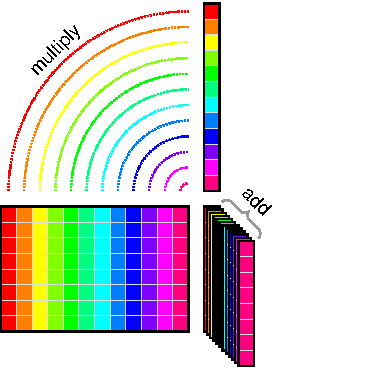
\includegraphics[width=0.6\textwidth]{figures/mv.pdf}
    \caption{A conceptual look at the linear layer. Each coloured band (“rainbow”) 
    handles a slice of the input multiplied by the matching slice of the weights ~\cite{githubdocs}.}
    \label{fig:mv}
\end{figure}
One can further simplify the multiplication \(\mathbf{A}\mathbf{x}\) by noting that
\emph{if \(\mathbf{x}[i]\) is zero, we skip column~\(i\) entirely.} 
In other words, \(\mathbf{A}\mathbf{x}\) becomes:
\[
\mathbf{A}\mathbf{x} \;=\; \sum_{\,i\;:\;\mathbf{x}[i]\neq0} 
   \bigl[\text{column } i\text{ of }\mathbf{A}\bigr] \cdot \mathbf{x}[i],
\]
which is extremely useful for a sparse \(\mathbf{x}\). 
Although \(W\) (or \(\mathbf{A}\)) may have tens of thousands of columns, 
engines only process those columns for features that are active in the current position.
\begin{figure}[H]
    \centering
    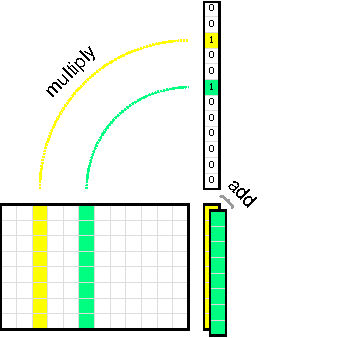
\includegraphics[width=0.6\textwidth]{figures/mvs.pdf}
    \caption{Skipping columns of \(\mathbf{A}\) for zero-valued inputs. 
    Only the columns corresponding to nonzero features in \(\mathbf{x}\) are processed ~\cite{githubdocs}.}
    \label{fig:skipcol}
\end{figure}
\paragraph{Clipped ReLU and Partial Updates}
After multiplying by \(W\), many NNUE implementations apply a \emph{clipped ReLU} 
activation to introduce non-linearity. In integer-based engines, this often includes 
a \emph{shift and clamp} so that intermediate sums remain within valid numeric ranges 
(e.g., 8-bit or 16-bit accumulators). By selectively updating only the neurons 
corresponding to changed squares, the engine avoids recalculating every feature on 
every move. In practice, two \emph{accumulators} store hidden-layer values for each 
side’s perspective (e.g., White vs.\ Black). When a piece moves from one square to 
another, the old location’s contribution is subtracted, the new location’s contribution 
is added, and the clipped/shifted ReLU ensures the layer remains both bounded and 
non-linear.



\begin{figure}[H]
    \centering
    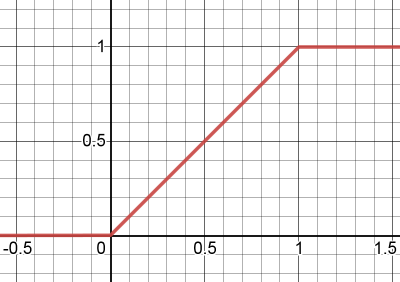
\includegraphics[width=0.6\textwidth]{figures/clipped_relu.png}
    \caption{After the linear layer, a clipped or shifted activation keeps integer 
    operations within limits, with only changed squares prompting recalculations ~\cite{githubdocs}.}
    \label{fig:mvs}
\end{figure}

\paragraph{Overall Pipeline}
Figure~\ref{fig:nnue_pipeline} shows an incremental NNUE flow. Each green node represents a piece-square feature, most of which remain constant on a given move. Hidden layers (yellow) combine weighted sums and clipped ReLU activations, while the final red output node yields a position evaluation. By performing small, targeted updates instead of a full forward pass every move, alpha-beta engines maintain high speed despite a neural-based evaluation.

\begin{figure}[H]
    \centering
    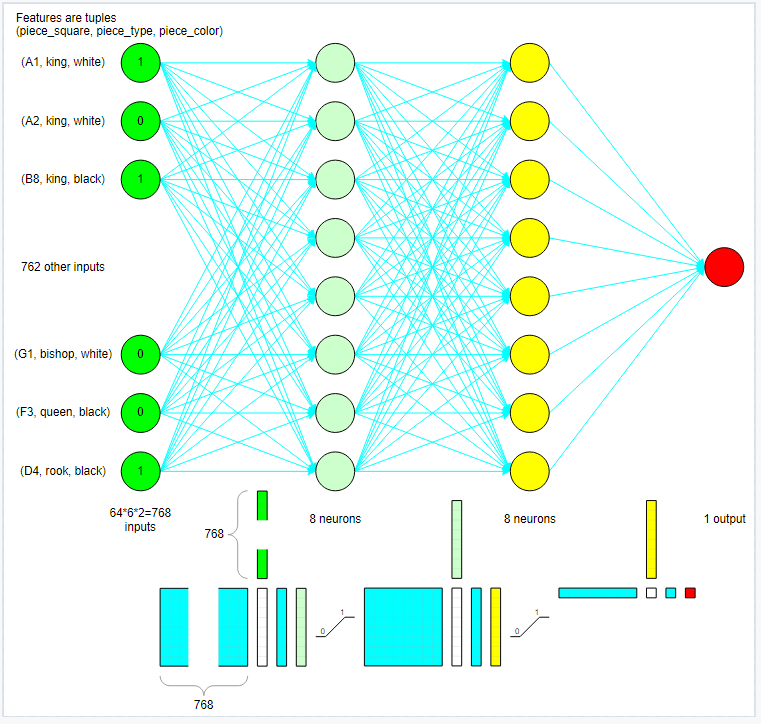
\includegraphics[width=0.8\textwidth]{figures/pipeline.png}
    \caption{A simplified NNUE pipeline: piece-square inputs (green) flow through 
    fully-connected hidden layers (yellow), yielding a single evaluation output (red) ~\cite{githubdocs}.}
    \label{fig:nnue_pipeline}
\end{figure}

\paragraph{HalfKP: Basic Piece-Square Mapping}
\label{sec:halfkp}

One of the earliest NNUE variants, \texttt{HalfKP}, focuses on \emph{piece-square
pairs} relative to each king’s position. It maintains two “perspectives": one for the side to move and another for the opposing side.
Each perspective can hold tens of thousands of binary features (for example,
\texttt{40960}), which feed into a \texttt{40960$\to$256} linear layer (the
\texttt{256} here can be any chosen number of neurons), followed by a clipped
ReLU activation.\medskip

\noindent
\textbf{Feature Index Computation.} In our implementation, each feature index is computed by:
\[
\begin{aligned}
p\_idx &= (\text{piece\_type}) \times 2 \;+\; \text{piece\_color},\\
\text{halfkp\_idx} &= \text{piece\_square} 
    \;+\;
    \bigl(p\_idx + (\text{king\_square} \times 10)\bigr)\times 64.
\end{aligned}
\]
The special case is when the king itself moves. Since \(\text{king\_square}\) appears in many feature indices, \emph{all} those features change and we must perform an accumulator refresh. Although more costly for king moves, this remains a rare event and keeps the overall number of updates per evaluation low.

\medskip

\noindent
\textbf{Partial Updates for Efficiency.} Although only a few input features change from move to move, we can exploit this sparsity by storing partial sums in the engine’s state (the “accumulators”). Recall that a linear layer effectively adds columns of a weight matrix based on which features are active. Instead of recomputing the entire first hidden layer, we do:
\begin{itemize}
    \item \textbf{Removed feature} (\(1 \to 0\)): \quad \emph{subtract} that feature’s column from the accumulator.
    \item \textbf{Added feature}  (\(0 \to 1\)): \quad \emph{add} that feature’s column to the accumulator.
\end{itemize}
A single move usually affects only one or two pieces (e.g.\ a capture, promotion, or normal displacement), so identifying changed features is straightforward. As a result, the incremental approach remains efficient even when combined with alpha-beta search.

\begin{figure}[H]
    \centering
    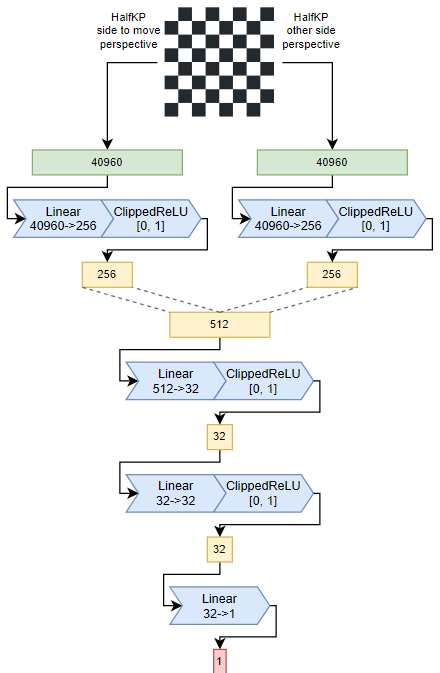
\includegraphics[width=0.6\textwidth]{figures/sfnn.png}
    \caption{An example \texttt{HalfKP} architecture ~\cite{githubdocs}.}
    \label{fig:halfkp_arch}
\end{figure}

\noindent  
In Figure~\ref{fig:halfkp_arch}, the network’s \emph{left block} corresponds to the accumulator for the side to move, while the \emph{right block} corresponds to the opposing side. Each block begins with a large binary input (e.g.\ \texttt{40960} features), encoding piece-square pairs relative to that side’s king. These features pass through a linear layer (\texttt{40960$\to$256}) and a clipped ReLU, producing a 256-dimensional output. The two 256-dimensional outputs (one per accumulator) are then concatenated into a 512-dimensional vector, which flows through additional fully-connected layers (e.g.\ \texttt{512$\to$32$\to$32$\to$1}) to yield a single scalar evaluation.

\medskip

By updating only the features that changed (e.g.\ a knight moving from c3 to e4), \texttt{HalfKP} greatly reduces overhead compared to a naive feed-forward pass. This incremental strategy is especially effective on CPU-based chess engines.


\paragraph{HalfKAv2: Refined Input Organization}
\label{sec:halfkav2}

\texttt{HalfKAv2} rearranges \texttt{HalfKP}’s piece-square indices to reduce collisions, where different squares might otherwise map to the same feature index. It uses \emph{buckets}, or separate weight sets, based on how many pieces remain on the board (e.g.\ special “endgame” weights). These refinements improve partial updates and adapt evaluations across different game phases.

As shown in Figure~\ref{fig:halfkav2}, the indexing layer is reorganized so that
each piece-square combination is mapped more distinctly. The diagram also
illustrates \emph{optional buckets}—in essence, separate weight matrices
specialized for different material levels (e.g., midgame versus endgame).
When the engine detects a transition (typically calculated via 
\((\mathrm{piece\_count} - 1) \div 4\)), it activates the relevant bucket to
make use of more specialized evaluation weights. This approach allows the
engine to adapt its heuristics based on how many pieces remain on the board
without altering the underlying feature index.
\medskip

\noindent
\textbf{Revised Feature Index Formula.}
A typical \texttt{HalfKAv2} approach avoids a separate king plane by merging white and black king categories. 
As shown below, the formula maps each non-king piece to one of 11 planes, flips squares for black’s perspective, 
and combines piece type, square, and king-square into a final index:

\[
\begin{aligned}
&\textbf{If } (\text{piece\_type} = 6) \;\rightarrow\; \text{index} = -1 \quad(\text{skip king}),\\
&p\_idx 
= (\text{piece\_type}-1)\times 2 
  \;+\; 
  \delta(\text{piece\_color\_white} \neq \text{is\_white\_pov}),\\
&\textbf{if } p\_idx=11 
  \;\rightarrow\; 
  p\_idx=10 \quad(\text{merge king plane}),\\
&sq\_o =
\begin{cases}
\text{sq}, & \text{if is\_white\_pov = true},\\
56 \oplus \text{sq}, & \text{if is\_white\_pov = false},
\end{cases}\\
&k\_sq\_o =
\begin{cases}
\text{king\_sq}, & \text{if is\_white\_pov = true},\\
56 \oplus \text{king\_sq}, & \text{if is\_white\_pov = false},
\end{cases}\\
&\text{index} 
= sq\_o 
  \;+\;
  (p\_idx \times 64)
  \;+\;
  (k\_sq\_o \times 64 \times 11).
\end{aligned}
\]

\noindent
\textbf{Explanation and Buckets.}
If the piece type equals \emph{king}, the formula returns \(-1\) to skip it. 
Otherwise, \(\mathrm{p\_idx}\) ranges from \(0\) to \(10\) after merging potential king categories. 
A perspective flip occurs when \(\mathrm{is\_white\_pov} = \text{false}\), using 
\(56 \oplus \text{square}\) to orient the board from Black’s viewpoint. 

\begin{figure}[H]
    \centering
    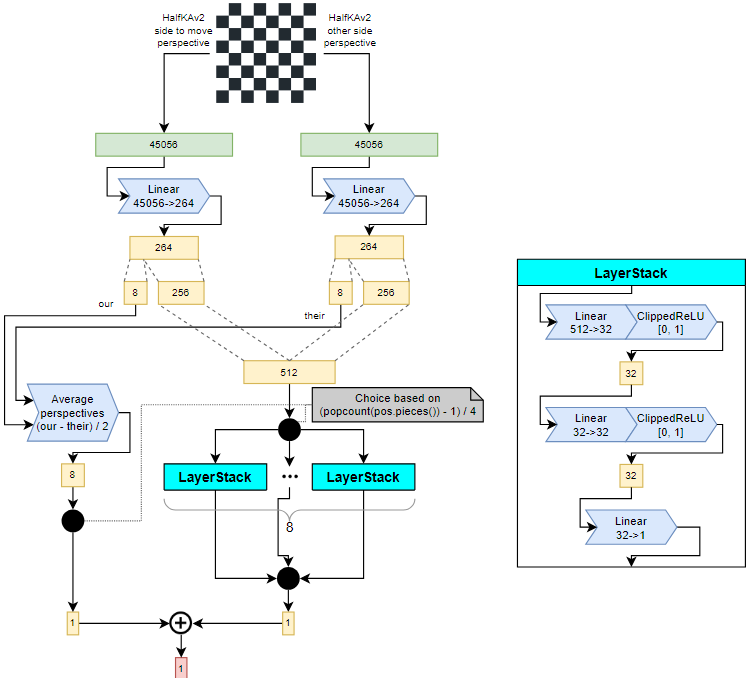
\includegraphics[width=1\textwidth]{figures/sfnn2.png}
    \caption{\texttt{HalfKAv2}: rearranged indices to minimize collisions 
    and optional buckets for variable piece counts. Each bucket (e.g.\ midgame, endgame)
    can hold its own specialized weight set, enabling more accurate evaluations 
    in different phases ~\cite{githubdocs}.}
    \label{fig:halfkav2}
\end{figure}

\paragraph{HalfKAv2\_hm: Mirrored or Hash-Map Variant}
\label{sec:halfkav2_hm}

\texttt{HalfKAv2\_hm} (sometimes referred to as “mirrored” or “hash map”) refines
indexing further by flipping or mirroring ranks and files. As illustrated in
Figure~\ref{fig:halfkav2_hm}, the board is mapped to feature indices in a more
compact way, effectively cutting the total number of indices in half. 

\medskip

\noindent
\emph{Horizontal mirroring} reflects each rank left-to-right around the
central vertical axis (files D/E). Squares on the a-file and h-file, for
example, are treated as “mirrors” of each other, yet still receive unique
identifiers. Compared to earlier \emph{board flipping} (inverting ranks
top-to-bottom), this method not only captures symmetrical positions but also
yields \emph{fewer overall indices}, reducing the size of any accumulators or
tables that track these features. As a result, incremental updates are much
faster, making \emph{horizontal mirroring} the more efficient choice for
handling symmetries.


\begin{figure}[H]
    \centering
    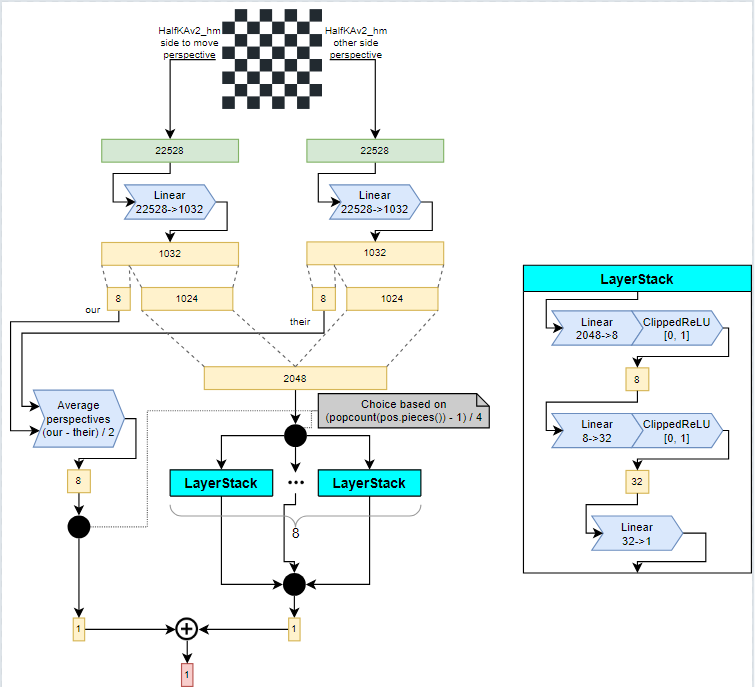
\includegraphics[width=1\textwidth]{figures/1.png}
    \caption{\texttt{HalfKAv2\_hm} uses mirrored or hashed rank/file references 
    to reduce collisions further. Here, horizontal mirroring reflects the board 
    left-to-right, while flipping inverts ranks top-to-bottom, improving partial 
    updates for symmetric positions ~\cite{githubdocs}.}
    \label{fig:halfkav2_hm}
\end{figure}


\paragraph{Practical Impact on Engines}
Historically, chess engines relied on hand-tuned heuristics (e.g.\ piece-square tables, king safety checks). NNUE replaces many of these with a learned approach, often discovering patterns humans did not explicitly encode. By combining incremental NNUE layers with alpha-beta, engines like \emph{Stockfish} achieve strong results in tournaments. This blend of sparse, partial updates and a machine-learned evaluation offers a robust yet efficient pipeline on regular CPUs.


\subsection{Chess Platforms and Visualization Tools}
\label{sec:chess_and_visualization}

Most popular chess engines, such as Stockfish or Lc0, run inside graphical interfaces (e.g., Arena, Cute Chess, SCID) that display the engine’s recommended move and a numerical evaluation \cite{stockfishdocs,lichessEngineIntegration,arenaDocs,cuTechessDocs,scidDocs}. While this setup helps users see which move is best, it does not show \emph{how} the engine arrives at that decision. Typically, there is no option to watch the internal search tree expand or see how each candidate move is evaluated at various depths.

Outside of chess, some interactive tools focus on \emph{pathfinding} rather than board-game search. For instance, \emph{MazeSolver} \cite{mazeSolverSite} allows users to place walls on a grid and then run algorithms like Breadth-First Search (BFS) or Depth-First Search (DFS), observing how the chosen algorithm explores the maze cell by cell. Similarly, \emph{PathfindOut} \cite{pathfindoutSite} provides a web interface for experimenting with various pathfinding methods, including Dijkstra’s Algorithm and A* (A-star). Although both sites offer a clear, step-by-step illustration of how nodes are visited and paths are formed, neither provides \emph{preloaded mazes} or \emph{standardized benchmark layouts} that could help users measure and compare algorithm performance in a consistent manner \cite{SomePathfindingDiscussion}. Instead, users must hand-draw obstacles or maze patterns each time, making quick demonstrations or controlled testing more difficult.

Meanwhile, typical chess interfaces focus on final engine outputs (for example, a numeric evaluation in centipawns) without revealing the move-by-move search process \cite{AlphaBetaTutorial}. While these outputs are sufficient for practical gameplay, they do not help learners or developers who want a deeper look at the algorithm’s decision-making. Although pathfinding visualizers demonstrate the \emph{benefit} of interactive, stepwise feedback, they often lack built-in benchmarks, and common chess GUIs omit visualization of the decision tree.

Summarizing these observations highlights two main gaps:
\begin{enumerate}
    \item \textbf{Absence of Benchmarks and Preloaded Mazes in Pathfinding Tools:}
    MazeSolver \cite{mazeSolverSite} and PathfindOut \cite{pathfindoutSite} rely on user-defined grids and lack standardized layouts or metrics, limiting consistent, repeatable tests for performance comparison.
    \item \textbf{No minimax visualizations:}
    Most chess platforms show only a final score or best move, without revealing how each node in the search tree is evaluated or pruned.
\end{enumerate}

Addressing these gaps could provide more accessible, instructive interfaces for both algorithmic learning and engine development. In subsequent sections, we will consider approaches that enable ready-made maze scenarios for consistent testing and expose the step-by-step searching logic in a chess engine.

\subsection{Hypothesis}
\label{sec:hypothesis}

Many maze-generation platforms lack strong visualization features, and they are
rarely combined with chess engines. Inspired by NNUE’s success in other projects,
this work aims to build a complete platform that merges maze generation and
visualization with an NNUE-enhanced Sunfish engine. The following questions guide
this study:

\begin{itemize}[label={}, leftmargin=1em]

\item \textbf{(a)} Does adding an NNUE-style network to the Sunfish engine lead
to a significant improvement in playing strength, compared to the original
heuristic-based method?

\item \textbf{(b)} Can creating a more advanced maze visualization tool boost
clarity, user engagement, and feature completeness beyond what is currently
offered?

\item \textbf{(c)} Could we develop a new tool that interactively visualizes minimax, making the algorithm more understandable?

\item \textbf{(d)} Is it feasible and beneficial to combine NNUE, enhanced maze
visualization, and a minimax visualizer into one platform, offering a unified set
of features to users?

\end{itemize}

These questions will be examined by measuring how much NNUE augmentation
improves the engine’s performance, along with evaluating user feedback on the
new visualization features.

\section{Background}
\label{sec:Background}

This section presents the core technologies and frameworks used in developing our application, spanning both the front-end and back-end. We also highlight the underlying chess engine algorithms and our chosen containerization strategy. 

\subsection{Languages, Frameworks, and Tools}
\subsubsection{Front-end}
When developing modern web applications, the primary front-end languages must run
in the browser, which generally narrows the choices to JavaScript or TypeScript (a typed superset of JavaScript)~\cite{ECMA}. However, front-end development also relies on foundational technologies such as HTML and CSS, standardized by the W3C, to structure and style web pages~\cite{W3C,MDNDocs}. 

In recent years, various \emph{front-end frameworks} (e.g.\ React, Angular, Vue) and build tools (e.g.\ Webpack, Babel) have emerged to simplify development and enhance performance~\cite{webpack,babel}. These tools enable developers to build \emph{single-page applications} (SPAs) that provide better user experience by dynamically rendering and updating page content without full page reloads. Additionally, package managers like \emph{npm} or \emph{yarn} streamline the process of installing and managing external libraries, making it easier to integrate third-party code~\cite{npmDocs,yarnDocs}.

\subsubsection*{JavaScript}
JavaScript is a high-level, dynamically typed language originally designed for adding
interactivity to web pages~\cite{ECMA,JSHistory}. It runs natively in the browser, making it a leading choice for front-end development. Over time, it has evolved through the ECMAScript standards (often referred to as ES6 or ES2015 and beyond), which introduced modern features such as arrow functions, classes, and modules. These enhancements enable more maintainable and modular code.

JavaScript uses an event-driven, single-threaded execution model, managed by the event
loop. This design allows for asynchronous operations via callbacks, promises, or \texttt{async/await}, ensuring responsive user interfaces~\cite{KyleSimpsonAsyncJS}. Although traditionally a client-side language, JavaScript is equally capable on the server side through platforms like Node.js, enabling full-stack development in a single language~\cite{nodeDocs}.

\subsubsection*{React}
React is a market-leading JavaScript library (though some developers call it a “framework”
due to its structured approach) created by Facebook (now Meta)~\cite{ReactDocs}. Its primary strength lies in its \emph{component-based architecture}, where UI elements are split into reusable components that manage their own \texttt{state}. When this state changes, React efficiently re-renders the affected components by leveraging a \emph{virtual DOM}. In contrast to “vanilla” JavaScript, where developers manually update the DOM, React’s virtual DOM automatically determines which parts of the real DOM need updating, minimizing unnecessary manipulations.

Additionally, React offers various \textit{Hooks} (such as \texttt{useState} and \texttt{useEffect}) that trigger re-renders under specific conditions~\cite{ReactHooksDocs}. These Hooks reduce the boilerplate typically found in class-based components, making React both flexible and powerful for building dynamic, responsive interfaces.

\subsubsection*{Tailwind CSS}
Tailwind CSS is a \emph{utility-first} framework that provides small, reusable classes for layout, spacing, colours, and more~\cite{TailwindDocs}. Unlike older frameworks like Bootstrap, it does not offer pre-built components or a default theme. Instead, developers can combine individual utility classes to build custom designs.

This approach works especially well in React applications, where you can place classes
directly in JSX, keeping your styles clear and consistent. Another benefit is the reduced risk of naming conflicts across different React components, since Tailwind’s classes are purpose-built for utilities rather than general styles. Tailwind also includes a configuration file that lets you enable only the classes you need, reducing your final CSS size and speeding up page loads.

\subsubsection*{Front-end Third-Party Libraries}
\paragraph{Chess.js}
Chess.js is a JavaScript library that provides chess rules, move generation, and board
validation~\cite{chessjs}. It supports features like check, checkmate, and move history tracking, simplifying the implementation of core game logic for browser-based applications.

\paragraph{React Flow}
React Flow is a library designed for interactive node-based UIs~\cite{reactflowDocs}. By abstracting away low-level details of draggable, zoomable views, it allows developers to quickly build complex flow diagrams. In this project, React Flow supports visual representations of algorithms or game-state transitions, enhancing user understanding.

\subsubsection{Back-end}
\subsubsection*{FastAPI}
FastAPI is a modern Python framework designed for building high-performance web APIs~\cite{fastapiDocs}. It leverages Python's \emph{async} features, enabling it to handle many simultaneous requests efficiently. One of FastAPI’s standout traits is its use of \emph{type hints}, which allow it to automatically generate detailed documentation and interactive Swagger/Redoc interfaces. This makes it straightforward to develop and test endpoints without writing extra code. In this project, FastAPI provides the back-end services for receiving user requests, handling logic, and returning responses in a clean, maintainable way.

To serve these applications, FastAPI typically runs on an ASGI server, such as \texttt{uvicorn}, which takes advantage of asynchronous execution to handle many simultaneous connections. This synergy between FastAPI and \texttt{uvicorn} makes it an excellent choice for back-end services in Python projects~\cite{uvicornDocs}.

\subsubsection*{PyTorch}
PyTorch is a popular Python library for deep learning, known for its \emph{dynamic computation
graph} and ease of use~\cite{pytorchDocs}. It integrates smoothly with NumPy, allowing developers
to switch between NumPy arrays and PyTorch tensors with minimal overhead. This flexibility makes
PyTorch especially convenient for experimenting with different neural network architectures.

In this project, PyTorch is used to implement and train an \textbf{NNUE} (Efficiently Updatable
Neural Network), a specialized network structure originally designed for chess and shogi engines.
NNUE leverages feature inputs that can be incrementally updated, reducing the computational cost
when board states change. PyTorch’s built-in \texttt{autograd} feature automates backpropagation,
while its robust \emph{GPU acceleration} shortens training time. Combined with a large community
and extensive documentation, PyTorch offers a practical foundation for integrating NNUE into
this AI-focused application.

\subsubsection*{Back-end Thirt-Party Libraries}
\paragraph{NumPy}
NumPy is a fundamental Python library for numerical computing, providing a powerful
\emph{multi-dimensional array} object along with tools for fast operations~\cite{Harris2020Array}. It
supports a wide range of data formats, making it straightforward to import and export datasets
in formats like CSV, TXT, and more specialized binary formats. This compatibility helps
streamline workflows by allowing different parts of a project—such as data preprocessing and
model training—to share the same array structures. Additionally, many scientific and machine
learning libraries (including PyTorch and Pandas) integrate seamlessly with NumPy, further
simplifying the development of data-driven applications.
\paragraph{python-chess}
The \emph{python-chess} library~\cite{python-chess} provides robust functionality for chess-specific
tasks such as board representation, legal move generation, and simple evaluation routines. It can
also interface with stronger engines via UCI, making it a convenient tool for building, testing, or
analyzing chess programs in Python.

\paragraph{collections}
The \emph{collections} module~\cite{python-collections} is part of the Python standard library and
offers specialized container datatypes such as \texttt{deque}, \texttt{Counter}, and \texttt{defaultdict}. 
These structures can improve both performance and code clarity in data manipulation tasks. 
For instance, \texttt{deque} enables efficient appends and pops from both ends of a list, 
while \texttt{defaultdict} simplifies handling of dictionary keys that may not yet be defined.

\subsection{Docker}
Docker is a containerization platform that allows applications to run in isolated environments
called \emph{containers}~\cite{DockerDocs}. Docker uses \emph{images}, which serve as blueprints
detailing all essential components and dependencies a container needs, forming the foundation from
which containers are created. A typical image is essentially a block of information containing the
operating system base, required libraries, and the application code. When an image is executed, it
creates a container (a lightweight instance) that runs the application consistently across different
systems.

In addition to images and containers, Docker provides a feature called \emph{volumes} to handle
persistent storage. Volumes let you store and manage data outside the container's filesystem,
simplifying updates or container replacement without losing data. By utilizing this functionality,
Docker ensures that the application is agnostic of the underlying machine. This approach greatly
enhances portability, as Docker images can be pushed to a registry or packaged into a \texttt{.tar}
file. These advantages are key factors making Docker one of the most popular choices for software
development and deployment.



\section{Design}
\label{sec:design}

Design is a key factor in building a practical, visually pleasing, 
and \emph{trustworthy} chess application. Good design improves how 
users see, understand, and interact with features. It can strengthen 
confidence in the system, ensure a smooth workflow, and reduce 
the cognitive load on users. In essence, a well-crafted design 
promotes \textbf{usability}, \textbf{engagement}, and \textbf{clarity}.

\subsection{Importance of a Clear Layout}
A simple, repetitive layout can quickly lose a reader’s attention. 
Conversely, \textbf{dynamic layouts} that balance text and images 
break large blocks of information into more manageable pieces, 
making the user experience more welcoming. Research indicates 
\cite{dombrowski2008layout} that alternating text and visuals 
(often called a \emph{zigzag} pattern) can reduce visual fatigue 
and boost content retention. Following ideas from 
Nielsen~\cite{nielsen2006usability}, this project also uses 
\textbf{keyword highlights}—for instance, marking key phrases 
(\texttt{NNUE} or \texttt{Minimax}) in \texttt{green} or 
\texttt{red}—to draw attention and guide the user’s eye.

\subsection{Layout-Driven Approach and Zigzag Highlights}
Tsumura et al.~\cite{tsumura2022layout} emphasize a \emph{layout-driven approach} 
to webpage reading, in which the structure, visual emphasis, and text-image 
placement guide how users (and screen readers) interpret content. 
Within this approach, the \emph{zigzag pattern} is especially useful 
for preventing visual monotony and directing attention . 
On larger screens, text typically appears on one side while an image 
or illustration occupies the opposite side. On smaller screens, 
these elements stack vertically to preserve readability.

Moreover, \textbf{color-coded keywords} (e.g., \texttt{text-green-500}) 
help emphasize terms like \texttt{NNUE} or \texttt{Minimax}, 
drawing the user’s focus immediately. These design choices reduce 
visual fatigue and highlight important concepts, aligning with the 
layout-driven principle of conveying structure through both text 
and visual arrangement.

\vspace{1em}
\noindent
\textbf{Example of a Zigzag Layout in Code.}  
Listing~\ref{lst:design_snippet} illustrates how 
\texttt{md:grid md:grid-cols-2} sets up a two-column 
layout for medium-sized screens, with classes such 
as \texttt{text-green-500} to emphasize crucial terms.

\begin{figure}[htb]
\centering
\begin{lstlisting}[language=HTML, breaklines=true, basicstyle=\small\ttfamily]
<section className="md:grid md:grid-cols-2 md:gap-12 items-center">
  <div>
    <h2 className="text-2xl font-bold mb-4">
      Understanding <span className="text-green-500">NNUE</span>
    </h2>
    <p className="text-gray-300 leading-relaxed">
      The <span className="text-green-500">NNUE</span> approach 
      offers more flexible and precise board evaluations...
    </p>
  </div>
  <div className="bg-gray-900 p-6 rounded-md shadow-lg">
    {/* Additional content or an image can appear here */}
  </div>
</section>
\end{lstlisting}
\caption{A React snippet showing a two-column layout (zigzag) and 
highlighted keywords (e.g., \texttt{NNUE} in green).}
\label{lst:design_snippet}
\end{figure}

\subsection{Screenshot and Visual Confirmation}
Figure~\ref{fig:design_screenshot} shows how this layout appears 
in the actual interface. If only one main image is available (or 
if multiple images look nearly the same), using a single best 
screenshot can effectively demonstrate how text and images 
alternate, preventing a dull or uniform look. Notably, highlighted 
keywords improve visibility of key features.

\begin{figure}[H]
    \centering
    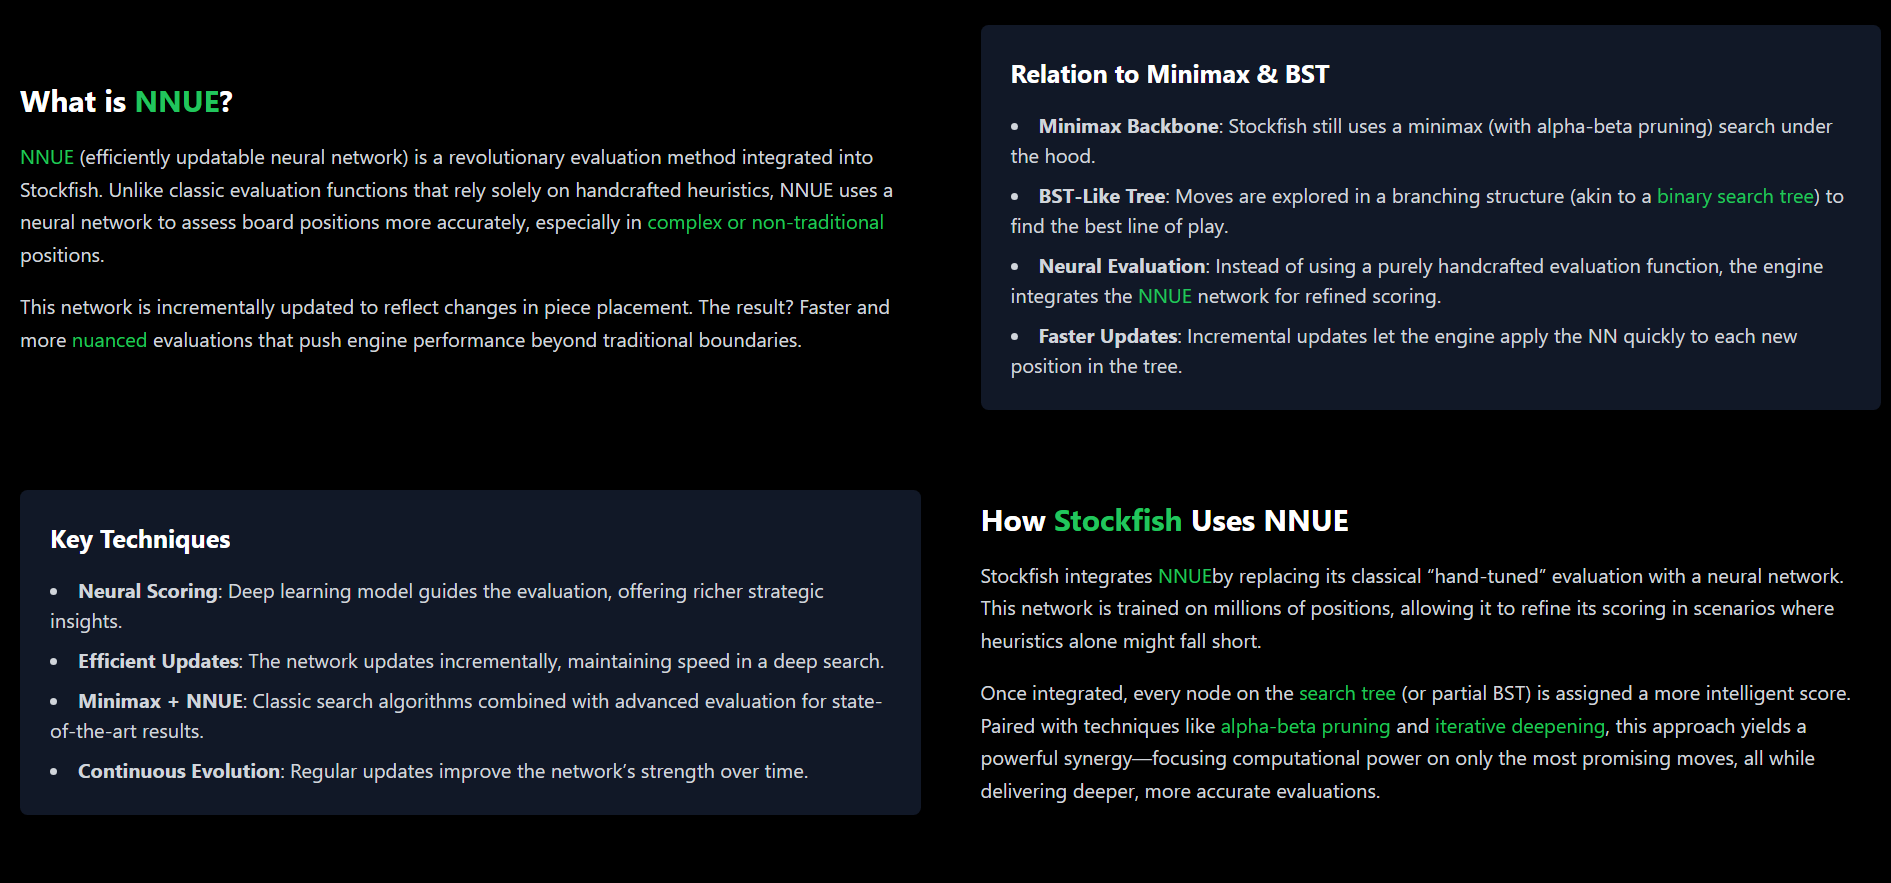
\includegraphics[scale=0.35]{figures/zigzag_interface.png}
    \caption{An example of the partial zigzag design. 
    Text is on one side, an image on the other, while 
    keywords such as \texttt{NNUE} appear in green 
    to attract focus.}
    \label{fig:design_screenshot}
\end{figure}

\subsection{Conclusion}
In summary, this project’s design approach centers on:
\begin{itemize}
    \item \textbf{Avoiding Repetition}: Alternating (zigzag) 
    or partially alternating text and images to keep viewers interested.
    \item \textbf{Emphasizing Key Terms}: Applying color highlights to 
    important labels like “\texttt{NNUE}.”
    \item \textbf{Responsive Layout}: Ensuring the layout scales gracefully 
    across different screen sizes.
    \item \textbf{Building User Trust}: Presenting information 
    in a structured, polished manner so users feel confident 
    in the application.
\end{itemize}

By adhering to this \emph{layout-driven approach}—balancing 
visual variety and carefully placed highlights—the design 
encourages consistent user focus, improves comprehension 
of crucial features, and fosters a more positive interaction experience.



\section{Architecture}
\label{sec:architecture}
\subsection{Overview}
\begin{figure}[H]
    \centering
    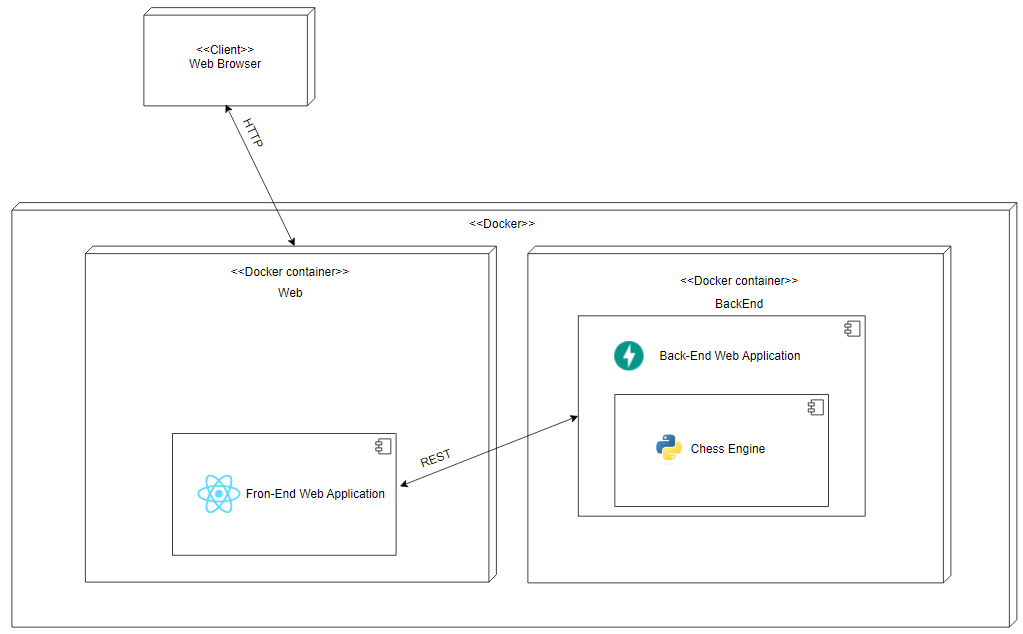
\includegraphics[width=1\textwidth]{figures/diagram1.png}  % adjust width as needed
    \caption{diagram illustrating the user’s browser interacting with 
    a front-end container and a back-end container, which houses the Chess Engine.}
    \label{fig:system-architecture}
\end{figure}

As shown in Figure~\ref{fig:system-architecture}, the system is composed of two Docker containers—
one for the front-end (React) and another for the back-end (FastAPI + NNUE). The user accesses 
the application through a standard web browser, sending HTTP requests to the front-end, which 
in turn communicates with the back-end via REST.




\subsection{Communication Flow}
Communication between the React front end and the FastAPI back end follows a straightforward RESTful request--response cycle over HTTP. Figure~\ref{fig:system-architecture} provides a high-level overview, while this subsection details how each endpoint fits into the application's workflow. Generally, users interact with buttons or pages in the React interface, triggering specific HTTP requests to the FastAPI server. The server processes these requests and returns the necessary data, which the front end uses to update the user interface.

\paragraph{Maze Endpoint}
\begin{itemize}
  \item \texttt{GET /api/maze}:
    \begin{itemize}
      \item \textbf{Purpose}: Generates a maze based on specified dimensions (\texttt{width}, \texttt{height}, and \texttt{tile}), then returns a text representation, with \texttt{0} indicating free space and \texttt{1} indicating a wall.
      \item \textbf{Usage}: The React client (e.g., a Maze page or component) requests a maze whenever the user clicks a “Generate Maze” button.
      \item \textbf{Flow}:
        \begin{enumerate}
          \item \textbf{Front end} sends \texttt{GET /api/maze?width=40\&height=20\&tile=2}.
          \item \textbf{Back end} calls \texttt{generate\_maze} and \texttt{convert\_maze\_to\_array}, then converts the resulting 2D array into a string.
          \item \textbf{Response} is returned as plain text, which the React client parses to display the maze layout.
        \end{enumerate}
    \end{itemize}
\end{itemize}

\paragraph{Chess Endpoints}
\begin{itemize}
  \item \texttt{POST /chess/makemove}:
    \begin{itemize}
      \item \textbf{Purpose}: Applies a user-submitted move (in UCI format) to the current chess position, then optionally runs a server-side chess engine for its own move suggestion.
      \item \textbf{Usage}: In the React chess page, the user selects and submits a move (e.g., \texttt{e2e4}), and the front end sends a JSON payload like \{\texttt{"move": "e2e4"}\}.
      \item \textbf{Flow}:
        \begin{enumerate}
          \item \textbf{Front end} sends \texttt{POST /chess/makemove} with the chosen move in JSON.
          \item \textbf{Back end} processes the move using \texttt{process\_move}, updating the \texttt{hist} (game history). It then calls the embedded chess engine, which accepts a UCI-style board representation to evaluate and possibly generate a response move.
          \item \textbf{Response} includes a status flag, any engine-generated move, and the updated FEN string so the front end can refresh the board state accordingly.
        \end{enumerate}
    \end{itemize}

  \item \texttt{POST /chess/reset}:
    \begin{itemize}
      \item \textbf{Purpose}: Restores the chessboard to the initial opening position.
      \item \textbf{Usage}: Triggered by a “Reset” or “New Game” button on the chess page.
      \item \textbf{Flow}:
        \begin{enumerate}
          \item \textbf{Front end} sends \texttt{POST /chess/reset}.
          \item \textbf{Back end} reinitialises the \texttt{hist} array to the default start position.
          \item \textbf{Response} returns a status flag plus the FEN of the new board, allowing the React client to render the reset position.
        \end{enumerate}
    \end{itemize}
\end{itemize}

\paragraph{CORS and Deployment Notes}
To enable local development, \texttt{CORSMiddleware} in FastAPI allows requests from \texttt{http://localhost:3000}, ensuring the React front end can communicate with the back end without cross-origin errors. For production, both parts can be containerised via Docker, allowing consistent environments across different machines.

\paragraph{Response Handling in React}
Regardless of the endpoint, the React client:
\begin{enumerate}
  \item Makes an HTTP request (with parameters or JSON data).
  \item Receives a response (plain text for the maze, JSON for chess moves).
  \item Updates the relevant component (e.g., Maze or ChessBoard) with the new state.
  \item Displays errors or invalid inputs using UI notifications if necessary.
\end{enumerate}

    By keeping the client-side focused on user interaction and display, and offloading maze generation and chess logic (including engine moves) to the server, this approach fosters a clear division of responsibilities in the application.

    \subsection{User Interface Structure}
    To facilitate both learning and direct experimentation, the web application offers two approaches:
    a \emph{guided path} for step-by-step exploration of concepts, and the option to \emph{jump directly}
    into specific visualization or gameplay features. Four main pages organize these capabilities:
    \begin{enumerate}
      \item \textbf{Home Page:} Introduces the project, providing general information and navigation links to the algorithm demos. It also lets users follow a guided path consisting of three detailed pages, each explaining:
        \begin{itemize}
          \item What Breadth-First Search (BFS) is and how it applies to maze traversal.
          \item How to build a basic NNUE (Neural Network Updatable Engine).
          \item How the minimax algorithm works, including its alpha--beta pruning variant.
        \end{itemize}
        This guided path gives novices a structured way to learn each concept before experimenting with live demos. Alternatively, users can skip the path and directly access any feature of interest.
      \item \textbf{Maze Visualization Page:} Demonstrates different pathfinding algorithms (including BFS) on a maze. Users can watch the process, adjust maze dimensions or generation parameters, \emph{or even construct a custom maze} by defining walls and starting points.
      \item \textbf{Minimax Traversal Page:} Allows users to step through a minimax search with alpha--beta pruning on a specific chess problem, illustrating how the algorithm chooses optimal moves.
      \item \textbf{Chess Page:} Lets users play against multiple engines such as Stockfish and Yanfish (the custom engine implementation).
    \end{enumerate}
    
    \subsubsection{Home Page}
    Serving as the application's entry point, the Home Page briefly explains the project's goals and functionalities. It also provides clear navigation links (e.g., a top menu or sidebar) to the other three pages. By offering a concise overview, this page ensures visitors can quickly choose between following the guided path or diving straight into any tool.
    
    \subsubsection{Maze Visualization Page}
    This page visualizes various pathfinding algorithms within randomly generated or custom-built mazes. It includes:
    \begin{itemize}
      \item \textbf{Algorithm Selection:} Users can choose BFS, DFS, Dijkstra, or A*.
      \item \textbf{Custom Maze Building:} Walls and pathways can be placed manually, allowing tailored scenarios.
      \item \textbf{Adjustable Maze Settings:} Parameters such as maze width or height can be changed to produce new layouts.
      \item \textbf{Interactive Controls:} Start, pause, or reset the pathfinding process; observe how each cell is explored.
      \item \textbf{Visual Feedback:} The traversal is animated step by step, helping users understand how these algorithms systematically uncover paths.
    \end{itemize}
    
    \subsubsection{Minimax Traversal Page}
    Here, users can explore how the minimax algorithm (with alpha--beta pruning) handles a specific chess problem:
    \begin{itemize}
      \item \textbf{Depth Selection:} Users can set the number of moves before running the algorithm.
      \item \textbf{Step-by-Step Explanation:} Each move can be examined using a control panel.
      \item \textbf{Interactive Visualization:} A visualized decision tree where users can double-click on a node to expand it, or fully expand the entire tree in one step.
    \end{itemize}
    
    \subsubsection{Chess Page}
    On the Chess Page, users can play interactive games against multiple engines:
    \begin{itemize}
      \item \textbf{Engine Selection:} Switch between Stockfish and Yanfish (the custom NNUE-enhanced engine) to compare playing styles.
      \item \textbf{Interface:} Displays the chessboard along with a move history, time controls, and a record of captured pieces.
    \end{itemize}
    
    \noindent
    Each of these four pages is accessible via a navigation bar at the top of the website. By separating
    functionality into modular subpages, users can easily focus on the specific algorithm or chess
    feature they wish to explore, while the underlying code remains cleaner and more maintainable.
    For further screenshots illustrating the interface, Appendix~\ref{sec:appendix}.
    
\subsection{Build}

To standardise environments and simplify deployment, we containerise both the front end and back end using Docker. 
Figure~\ref{fig:system-architecture} shows that each component runs in its own container:

\begin{itemize}
  \item \textbf{Front end (React):} We use a \texttt{Dockerfile} based on an Alpine-based Node image. After installing dependencies and building the production bundle, the container serves the compiled files. Alpine Linux provides a smaller footprint, reducing overall image size.

  \item \textbf{Back end (FastAPI + NNUE):} We use a \texttt{Dockerfile} based on an Alpine-based Python image. It installs libraries such as FastAPI, PyTorch, and any NNUE-specific packages, then launches \texttt{uvicorn}. Using Alpine reduces image bloat and streamlines resource usage.
\end{itemize}

Docker Compose is a YAML-based configuration tool that allows you to define and manage multiple containers for a single application. Instead of running separate Docker commands, you place all relevant settings—such as build instructions, environment variables, and port mappings—into a single file, typically called \texttt{docker-compose.yml}. This setup simplifies both development and deployment by letting you use one command (\texttt{docker-compose up}) to start all services at once.

\begin{lstlisting}[language=bash,caption={docker-compose.yml},label={lst:docker-compose at project root}]
version: "3.8"

services:
  BackEnd:
    build: .
    container_name: "fastapi_app"
    restart: "always"
    ports:
      - "8000:8000"
  Web:
    build:
      context: "./my-project"
    container_name: "frontend_app"
    restart: "always"
    ports:
      - "3000:3000"
    depends_on:
      - "BackEnd"
    environment:
      - REACT_APP_API_BASE_URL="http://localhost:8000"
\end{lstlisting}
\section{Implementation}
Having established the theoretical underpinnings and high-level design in previous chapters, we now turn to the practical side: the code. This section is divided into three parts. First, we walk through the neural network (NNUE) evaluation framework and its role in enhancing the chess engine’s strength. Second, we unveil the backend, which orchestrates data flow and enforces game rules. Finally, we showcase the frontend implementation, illustrating how users interact with the engine’s capabilities through a clean and responsive interface.
\subsection{NNUE Model}
\label{subsec:nnue_model}

The NNUE (Neural Network-based Underestimated Evaluation) model is central to this project, as noted in the hypothesis section \ref{sec:hypothesis}. The core idea is to develop a platform that brings together various visualization tools and integrates a chess engine enhanced by NNUE. By leveraging NNUE, the goal is to achieve more accurate position evaluations and stronger overall gameplay compared to traditional heuristic-based methods.

\subsubsection{NNUE Implementation}
\label{subsubsec:nnue_implementation}

This project employs the HalfKP architecture, one of the earliest NNUE-based designs used in Stockfish. Because training a model to reach grandmaster-level performance is time-consuming and requires extensive resources, we utilize pre-existing weights from a previously established neural network. To ensure consistency and correctness, we replicate the same operations that were used in the original training pipeline (Figure \ref{fig:halfkp_arch}). The key steps are:

\begin{itemize}
    \item Implement a feature transformer that calculates indices for each board position and generates an accumulator, enabling efficient updates.
    \item Construct a neural network that adheres exactly to the original HalfKP design.
    \item Integrate the neural network into the existing Sunfish chess engine.
\end{itemize}

This approach allows the project to achieve a competitive level of strength in position evaluation and move generation without incurring the high costs of training a new network from scratch.

\subsubsection*{Accumulator}
The HalfKP approach (Section \ref{sec:halfkp}) relies on an accumulator to handle feature transformations efficiently. By storing intermediate computations, the accumulator enables faster updates whenever a board state changes. This is particularly useful for searching through a large number of positions in the course of a chess engine's operation.

To implement this functionality, a \texttt{MyAccumulator} class was created in Python. This class leverages several libraries:
\begin{itemize}
    \item \texttt{chess} to represent and manipulate chess positions,
    \item \texttt{numpy} for efficient numerical operations, and
    \item \texttt{pytorch} for neural network integration.
\end{itemize}

\begin{lstlisting}[language=Python, caption={Part 1: Initialization of NNUEAccumulator}, label={lst:accumulator}, basicstyle=\footnotesize\ttfamily,breaklines=true]
class NNUEAccumulator:
    def __init__(self, 
                 weights_file="engines/weights/transformer_weights.npy", 
                 bias_file="engines/weights/transformer_bias.npy"):
        # Load the transformer's embedding weights and bias
        self.weights = np.load(weights_file)  # shape (41024, 256)
        self.bias = np.load(bias_file)        # shape (256,)

        # Validate shapes to ensure they match the expected dimensions
        assert self.weights.shape == (DEFAULT_NUM_FEATURES, FEATURE_TRANSFORMER_HALF_DIMENSIONS)
        assert self.bias.shape == (FEATURE_TRANSFORMER_HALF_DIMENSIONS,)

        # Initialize accumulator storage (batch dimension of 1, size of 512)
        self.accum = np.zeros((1, 512))
\end{lstlisting}
\paragraph{Explanation}
In Listing~\ref{lst:accumulator}, the constructor method loads the pre-trained weights and biases, checks their shapes against constants (such as \texttt{DEFAULT\_NUM\_FEATURES} and \texttt{FEATURE\_TRANSFORMER\_HALF\_DIMENSIONS}), and initializes a zeroed accumulator that will be updated incrementally after each move.
\begin{lstlisting}[language=Python, caption={Part 2: The update method snippet }, label={lst:accumulator_update}, basicstyle=\footnotesize\ttfamily,breaklines=true]
    def update(self, accum, turn, move, kings):
        """Incrementally update the accumulator for a new position."""
        from_sq = move[0]
        from_pc = move[1]
        to_sq   = move[2]
        to_pc   = move[3]

        our_king, opp_king = (kings[0], kings[1]) if turn else (kings[1], kings[0])

        # Create a new array matching the shape of the existing accumulator
        self.accum = np.empty_like(accum)

        # Calculate indices for the piece being moved
        index_from_w_perspective = self.make_halfkp_index(
            turn, self.orient(turn, our_king), from_sq, from_pc
        )
        index_from_b_perspective = self.make_halfkp_index(
            not turn, self.orient(not turn, opp_king), from_sq, from_pc
        )

        # If a capture or promotion occurs, calculate indices for those scenarios
        if to_pc is not None:
            index_to_w_perspective = self.make_halfkp_index(
                turn, self.orient(turn, our_king), to_sq, to_pc
            )
            index_to_b_perspective = self.make_halfkp_index(
                not turn, self.orient(not turn, opp_king), to_sq, to_pc
            )

        # Handle promotion cases for pawns
       

       ...
        # Update accumulators for both color perspectives
        self.accum[0][:256] = accum[0][256:512] \
                              + self.weights[index_to_b_perspective_new] \
                              - self.weights[index_from_b_perspective]
        self.accum[0][256:512] = accum[0][0:256] \
                                 + self.weights[index_to_w_perspective_new] \
                                 - self.weights[index_from_w_perspective]

        # Subtract weights for captured piece if applicable
        if to_pc is not None:
            self.accum[0][:256] -= self.weights[index_to_b_perspective]
            self.accum[0][256:512] -= self.weights[index_to_w_perspective]

        return self.accum
\end{lstlisting}

\paragraph{Explanation} 
In Listing~\ref{lst:accumulator_update}, the \texttt{update} method performs an incremental adjustment of the accumulator to reflect the latest move on the chessboard. First, it extracts the relevant details of the move:
\begin{itemize}
  \item \texttt{from\_sq}: The square the piece is moving from
  \item \texttt{from\_pc}: The piece on \texttt{from\_sq}
  \item \texttt{to\_sq}: The square the piece is moving to
  \item \texttt{to\_pc}: The piece on \texttt{to\_sq} (if any), used to detect captures or promotions
\end{itemize}

Next, it determines whose move it is by setting \texttt{our\_king} to the current mover’s king and \texttt{opp\_king} to the opponent’s king. A fresh \texttt{accum} array is created with \texttt{np.empty\_like} to store updated feature values. The method then calculates the feature indices for the moved piece (from both White’s and Black’s perspective) using \texttt{make\_halfkp\_index} \ref{lst:accumulator_utilities}, which converts a piece-specified square into a unique index for the HalfKP feature set.

If a capture or promotion occurs, the code computes additional indices to account for the new piece occupying the square (\texttt{to\_pc} or a promoted piece), as well as to remove any influence of the captured piece. Pawn promotions involve substituting the moved pawn with a queen piece (unless you alter it to handle other promotion cases) and calculating corresponding indices for both color perspectives.

The accumulator is updated for each half of its array: indices \texttt{[0:256]} represent Black’s perspective, and indices \texttt{[256:512]} represent White’s. In both ranges, the method:
\begin{enumerate}
  \item \textbf{Adds} the weights of any newly occupied square (promotions or regular moves),
  \item \textbf{Subtracts} the weights of the old square if the piece moved away or was captured,
  \item \textbf{Repositions} the piece by shifting its contribution from the source index to the destination index.
\end{enumerate}
Finally, if \texttt{to\_pc} is not \texttt{None}, meaning a capture happened, the contribution of the captured piece is removed from both perspectives by subtracting its corresponding weights.

This incremental approach ensures that only the portions of the feature vector changed by the move are recalculated, saving computation time. Instead of rebuilding the entire feature set from scratch, the method selectively applies additions or subtractions to reflect the new board state. The updated \texttt{accum} is returned for use in subsequent neural network evaluations, allowing the chess engine to efficiently evaluate each move in the game with minimal overhead.

\begin{lstlisting}[language=Python, caption={Part 3: Utility methods for orientation and index computation}, label={lst:accumulator_utilities}, basicstyle=\footnotesize\ttfamily,breaklines=true]
    def get_halfkp_indices(self, board: chess.Board):
        """Compute indices for all pieces on the board from both perspectives."""
        result = []
        is_white_pov = board.turn

        for turn_state in [board.turn, not board.turn]:
            indices = []
            for sq, piece in board.piece_map().items():
                if piece.piece_type == chess.KING:
                    continue
                indices.append(
                    self.make_halfkp_index(turn_state, 
                                           self.orient(turn_state, board.king(turn_state)), 
                                           sq, piece)
                )
            result.append(indices)

        return np.array(result, dtype=np.intp)

    @staticmethod
    def orient(is_white_pov: bool, sq: int) -> int:
        """Flip or retain square indexing based on side to move."""
        return (63 * (not is_white_pov)) ^ sq

    @staticmethod
    def make_halfkp_index(is_white_pov: bool, king_sq: int, sq: int, p: chess.Piece) -> int:
        """Combine orientation, piece-square encoding, and king-square indexing for HalfKP."""
        return NNUEAccumulator.orient(is_white_pov, sq) \
               + PieceSquare.from_piece(p, is_white_pov) \
               + PieceSquare.END * king_sq
\end{lstlisting}

In essence, \texttt{MyAccumulator} captures the relevant board features and transforms them into a format suitable for the neural network. Because each move in a chess game typically alters only a few squares, this approach allows updates to be carried out incrementally rather than computing all features from scratch.

\subsubsection*{NNUE}
\label{subsec:nnue_net}

While the accumulator focuses on efficiently tracking board features, the NNUE network itself leverages these features to evaluate positions. This network is built using the PyTorch library, allowing for straightforward model definition, training, and inference. By combining the HalfKP feature representation with a compact yet expressive feed-forward architecture, the network can efficiently process positional information and deliver accurate evaluations. 

\begin{lstlisting}[language=Python, 
                   caption={A simplified PyTorch implementation of the NNUE network structure}, 
                   label={lst:nnue_network},
                   basicstyle=\footnotesize\ttfamily,
                   breaklines=true]
class MyNNUE(nn.Module):
    def __init__(self):
        super(MyNNUE, self).__init__()
        self.layer1 = nn.Linear(512, 32)
        self.layer2 = nn.Linear(32, 32)
        self.output_layer = nn.Linear(32, 1)
        self.relu = nn.ReLU()
        self.load_extracted_weights()

    def forward(self, x):
        x = self.relu(self.layer1(x))
        x = self.shift_and_clamp_torch(x)
        x = self.relu(self.layer2(x))
        x = self.shift_and_clamp_torch(x)
        x = self.output_layer(x)
        return x  # shape (batch_size, 1)

   
\end{lstlisting}

\paragraph{Explanation}
The \texttt{MyNNUE} class follows a design similar to one of the early Stockfish neural networks. It includes two hidden layers, each with 32 neurons, and a final output layer that produces a single evaluation score. Between each layer, the \texttt{shift\_and\_clamp\_torch} function (discussed in Section~\ref{lst:shift_clamp}) ensures intermediate activations remain within a limited integer range, aligning with the integer-based arithmetic common in many NNUE engines. Additionally, the method \texttt{load\_extracted\_weights} inserts pretrained weights and biases directly into each layer, allowing this network to immediately leverage a previously optimized model. By structuring the network in this way, we can achieve a balance of simplicity, speed, and accuracy while still preserving the benefits of an NNUE-style incremental update system.


\subsubsection*{Shift and Clamp Logic}
Clamping prevents activations from growing too large or falling below a minimum value, while shifting can help align outputs with subsequent layers in an integer-based or limited-precision environment.

\begin{lstlisting}[language=Python,
                   caption={Example of a shift and clamp step},
                   label={lst:shift_clamp},
                   basicstyle=\footnotesize\ttfamily,
                   breaklines=true]
def shift_and_clamp_torch(self, x: torch.Tensor) -> torch.Tensor:
        """Bit-shifts and clamps values to [0, 127] while ensuring correct data types."""
        x = x.to(torch.int32)  # Convert to int32 before bit-shifting
        x = x >> SHIFT  # Apply bit-shift
        x = torch.clamp(x, CLAMP_MIN, CLAMP_MAX)  # Clamp to [0, 127]
        return x.to(torch.float32)  # Convert back to float32 for the neural network
\end{lstlisting}

\paragraph{Explanation}
Listing~\ref{lst:shift_clamp} demonstrates how a “shift and clamp” operation might look in a PyTorch-based NNUE setting. The \texttt{tensor} (which could be the output of a hidden layer or an accumulation step) is first shifted by a fixed amount to reduce its magnitude. This is often done in environments where integer arithmetic is used for performance or hardware constraints. Next, \texttt{torch.clamp} enforces a minimum and maximum value to prevent numerical overflow or excessively negative values. By maintaining outputs within a controlled range, we reduce precision loss and ensure the network’s evaluations remain stable.


    \subsubsection{Evaluation in the Search Loop}
    \label{sec:integration}
    This project integrates an NNUE-based evaluation into the Sunfish chess engine in a manner reminiscent of older Stockfish versions that initially relied on NNUE only at leaf nodes. Specifically, the \texttt{MyNNUE} class is invoked to generate evaluations at depth zero, leaving the deeper layers of the search to use Sunfish’s traditional heuristic evaluation and pruning mechanisms. This hybrid approach provides several benefits:

\begin{itemize}
  \item \textbf{Incremental NNUE Adoption:} By limiting NNUE calls to leaf nodes, the engine avoids performing expensive neural network evaluations at every depth, thus keeping computational overhead manageable.
  \item \textbf{Preservation of Proven Heuristics:} Deeper search layers still rely on well-tested heuristic rules, ensuring that pruning logic and move ordering—key components of Sunfish’s design—remain stable and effective.
  \item \textbf{Accumulator-Based Updates:} The \texttt{MyNNUE} class also employs an accumulator, which constructs and incrementally updates a 512-dimensional feature vector. When moving from one leaf node to another, only the parts of the board state that have changed get recomputed, reducing the cost of recalculating features from scratch.
\end{itemize}

In practice, when the engine explores a position at a leaf node (i.e., a position where depth $= 0$ or quiescence search ends), it instructs the accumulator to provide a current feature vector. This vector is then passed to the neural network in \texttt{MyNNUE}, which returns an evaluation score. That score is incorporated into the search’s alpha-beta logic to finalize a leaf evaluation. At deeper search levels, Sunfish’s existing, well-understood material/positional heuristics continue to guide move ordering, pruning, and extensions. This incremental, leaf-focused adoption of NNUE allows the engine to benefit from more accurate evaluation where it matters most—at terminal nodes—while avoiding the overhead of a full-scale neural network call on every position in the search tree.
\begin{lstlisting}[language=Python, caption={Refined Sunfish Searcher Code snippet with NNUE Integration}, label={lst:searcher_nnue}, basicstyle=\footnotesize\ttfamily, breaklines=true]
# Inside the Searcher class

# Instantiating the NNUE network
nnue = MyNNUE()

# Helper function to clamp and convert our accumulator for NNUE
def process_accum_for_nn(accum: np.ndarray) -> torch.Tensor:
    processed = np.clip(accum, CLAMP_MIN, CLAMP_MAX)
    return torch.tensor(processed, dtype=torch.float32)

# ...
# Later in the 'bound' method, we compute the leaf evaluation.
if depth == 0:
    if not self.use_classical:
        with torch.no_grad():
            x = process_accum_for_nn(cur_accum)  # shape: [1, 512] float32
            score_tensor = nnue(x)
        raw_score = int(score_tensor.item())
        score = (((raw_score // 16) * 100) // 208)
        print(score)
    else:
        score = pos.score

    # Return the leaf evaluation
    yield None, score

# ...
# Setting up and maintaining the accumulator
nnue_accum = NNUEAccumulator()
cur_accum = np.empty([1, 512], dtype=np.float32)  # Avoid direct changes to root

if not self.use_classical:
    if accum_up:
        # Recalculate entire accumulator if the king has moved or there's a special update needed.
        board = chess.Board(renderFEN(pos))
        turn = board.turn
        kings = (board.king(turn), board.king(not turn)) if turn else (board.king(not turn), board.king(turn))
        ind = nnue_accum.get_halfkp_indices(board)

        cur_accum[0][:256] = np.sum(nnue_accum.weights[ind[0]], axis=0)
        cur_accum[0][256:] = np.sum(nnue_accum.weights[ind[1]], axis=0)
        cur_accum[0][:256] += nnue_accum.bias
        cur_accum[0][256:] += nnue_accum.bias

        accum_up = False
    else:
        # Incremental update if only one piece has moved.
        if move_prev:
            move_chess = chess_move_from_to(pos_prev, move_prev)
            turn = False if pos_prev.board.startswith('\n') else True
            cur_accum = nnue_accum.update(accum_root, turn, move_chess, kings)
        else:
            # Handle null moves by swapping the two halves of the accumulator
            cur_accum[0][0:256] = accum_root[0][256:]
            cur_accum[0][256:] = accum_root[0][0:256]
\end{lstlisting}

\paragraph{Explanation}
In Listing~\ref{lst:searcher_nnue}, the \texttt{bound} method checks if \texttt{depth == 0} and, if so, uses \texttt{MyNNUE} to evaluate the position. By limiting neural network inferences to leaf nodes, the engine avoids excessive overhead. Meanwhile, \texttt{NNUEAccumulator} maintains a 512-dimensional feature vector. Depending on whether a king move or null move has occurred, the code either rebuilds the entire feature vector or uses \texttt{update} to adjust only the parts affected by the last move. This incremental approach reduces unnecessary recalculations and preserves the efficiency of Sunfish’s search, while still benefiting from NNUE’s strong evaluation at critical leaf positions.

  

\subsection{Backend Implementation}
The backend server in this project is designed to be straightforward yet versatile. As outlined in Section~\ref{sec:architecture}, it relies on \texttt{FastAPI} to manage server-side logic and client communications. One of the key design principles is to keep configuration minimal. Since the system does not require user authentication or persistent database storage, its core functionality depends almost entirely on \texttt{FastAPI} and a simple CORS setup, with no additional middleware or specialized libraries needed.

Several endpoints handle specific operations: Chess Move Submission, Maze Generation, and Game Reset. When a user submits a chess move in UCI format (for example, \texttt{e2e4}), the server updates the internal game state and returns the resulting position in FEN notation. This approach keeps the backend flexible by using well-known chess notation standards. The Maze Generation endpoint employs a depth-first search (DFS) with backtracking to produce a random maze, then serves the final result as either a text-based grid or a PNG image. By providing multiple content types in its responses, the backend demonstrates how \texttt{FastAPI} can serve diverse data formats with minimal overhead. A dedicated Game Reset endpoint reinitializes the chess position, allowing new games to start without restarting the server.

A notable component of this design is the DFS-based Maze Generation. Every cell in the maze starts with all four walls intact. A random cell is selected as the starting point and marked as visited. The algorithm uses a stack to track the path: at each step, it picks a random neighbor that has not been visited, removes the shared wall between the current cell and that neighbor, and proceeds until every cell has been visited exactly once. This guarantees a single connected path through all cells without cycles, ensuring that each maze remains unique. The final structure is then translated into text or a PNG image for convenient retrieval by the client.

Central to the maze generation is the \texttt{Cell} class, which encapsulates the logic for each grid location. A \texttt{Cell} stores its coordinates \texttt{(x, y)} as well as a dictionary of walls indicating whether each side (\texttt{top}, \texttt{right}, \texttt{bottom}, \texttt{left}) is still intact. It also features a boolean flag, \texttt{visited}, to indicate whether the maze-generation process has already included that cell in the path. Two methods, \texttt{check\_cell} and \texttt{check\_neighbors}, handle neighbor validity: \texttt{check\_cell} returns \texttt{None} if given invalid coordinates or the corresponding cell otherwise; \texttt{check\_neighbors} collects all valid, unvisited neighbors and then randomly selects one to continue carving passages. Once a path is established between two neighboring cells, their shared walls are removed, and both cells become part of the same contiguous corridor.

The backend itself runs on \texttt{uvicorn}, a high-performance ASGI server. By default, it listens on \texttt{127.0.0.1:8000}, which makes local testing straightforward and deployment to ASGI-compatible hosts simple. For chess functionality, a global list, \texttt{hist}, keeps track of all positions, updating whenever a move is submitted. If the user requests an engine move, the backend calculates and returns it in standard notation. By employing established formats such as FEN for board positions and UCI for moves, the backend ensures seamless compatibility with diverse client applications.


In summary, the combination of \texttt{FastAPI} and a straightforward DFS-based maze-generation algorithm creates a simple yet flexible backend. The \texttt{Cell} class ensures the maze construction process is well-structured, while returning data in multiple formats (JSON, text, images) highlights the adaptability of the system. This design is particularly suited to a lightweight frontend that needs immediate, clear data responses and minimal setup on the server side.
\begin{figure}[ht]
  \begin{center}
    \begin{minipage}{0.4\linewidth}
      \begin{lstlisting}[numbers=none,frame=none,basicstyle=\ttfamily\footnotesize,breaklines=true]
backend
|   endpoint.py
|   maze.png
|   maze.txt
|   __init__.py
|   ...
+--- engines
|   |   1.py
|   |   ...
|   \--- __pycache__
|       |   ...
|       \--- numpy_weights
|               ...
\--- tests
    |   test_sunfish.py
    \--- __pycache__
            ...
      \end{lstlisting}
    \end{minipage}
  \end{center}
  \caption{Simplified project directory structure }
  \label{fig:directory-structure}
\end{figure}


  \subsection{Frontend Implementation}

\label{sec:frontend}

The user interface is built with React (JavaScript) as the core framework, and Tailwind CSS for styling. Each page is implemented as a standalone React component consisting of multiple sub-components that collaborate to provide desired functionalities while maintaining clarity and clean code. We also leverage well-established libraries such as react-router (for seamless navigation) and \texttt{react-flow} (for interactive flow diagrams), installing and managing these dependencies via \texttt{npm}.

\begin{figure}[ht]
  \begin{center}
    \begin{minipage}{0.5\linewidth} % Adjust this width as needed
\begin{lstlisting}[numbers=none,frame=none,basicstyle=\ttfamily\footnotesize,breaklines=true]
.
|   Dockerfile
|   README.md
|   package-lock.json
|   package.json
+--- src
|   |   App.css
|   |   App.js
|   |   App.test.js
|   |
|   +--- components
|   |   |   ChessGamePage
|   |   |   DecisionTreePage
|   |   |   Header.jsx
|   |   |   HomePage.css
|   |   |   HomePage.jsx
|   |   |   MazeSolvingPage
|   |   |   MinimaxPage
|   |   |   NnnuePage
|   |   |   bstPage
|   |   |   engine
|   |   \--- toberemoved
|   |
|   |   index.css
|   |   index.js
|   \--- setupTests.js
\--- tailwind.config.js
\end{lstlisting}
    \end{minipage}
  \end{center}
  \caption{A simplified version of the project's directory structure.}
  \label{fig:directory-structure1}
\end{figure}

  \subsubsection{Navigation}

Navigation in the frontend uses \texttt{react-router-dom} to allow users to switch between different parts of the application without reloading the entire page. This setup makes transitions fast and enables the interface to update its content seamlessly. A single file, \texttt{App.js}, maps each URL path to a React component under \texttt{components/}.

Each major feature or page has its own folder and entry point, keeping the code organized. For example: \begin{itemize} \item \texttt{components/HomePage.jsx} holds the homepage layout. \item \texttt{components/MazeSolvingPage/MazeSolvingPage.jsx} includes maze-related features and visuals. \item \texttt{components/ChessGamePage/ChessGamePage.jsx} manages the chess interface and coordinates with the backend. \item \ldots \end{itemize}

From a user’s perspective, each page is accessed by a unique path (e.g., \texttt{/maze} for the maze solver, \texttt{/chess} for the chess interface). \texttt{react-router-dom} checks the requested path and seamlessly loads the correct component. Because the routing is handled on the client side, the experience feels smooth compared to a full page reload.

A shared header at the top level maintains a consistent layout across all pages. As the application grows, it can be split into sub-routes or nested routes to handle larger sections. Keeping the routing logic in \texttt{App.js} also makes adding or modifying pages straightforward.

    \subsubsection{Maze Visualization}

Our maze is presented as a grid of cells, each of which can be a wall 
(\texttt{1}) or an open space (\texttt{0}). When we fetch the raw maze data 
from the backend, we split it into lines and transform it into a 
two-dimensional array, which we refer to as \emph{grid}. This \emph{grid} 
helps the frontend recognize walls versus walkable paths.

To show the internal steps of a search algorithm (like DFS or BFS), we record 
a series of “events” in a dedicated array, which we call \emph{dfsEvents} 
for Depth-First Search or \emph{bfsEvents} for Breadth-First Search. Each 
entry in this array includes the row and column of the cell, plus whether 
the search is \emph{'visiting'} or \emph{'backtracking'}. We store a 
\emph{step} index in React state, indicating how many events have been 
processed so far. By incrementing \emph{step} one unit at a time (via a 
small time delay), the visualization updates cell by cell, letting us see 
the search progress in “real time.”

For coloring, walls remain black, while visited path cells are highlighted 
in distinct colors depending on their status. If a cell is on the current 
search path, it appears more vividly (for instance, red), and if it’s 
already explored and removed from the path (\emph{'backtracked'}), it might 
appear in a lighter shade (like light blue). We also mark the \emph{start} 
cell with an \texttt{S} and the \emph{end} cell with an \texttt{E}. This 
color-coding helps illustrate the search’s forward movement and backtracking 
phases, offering a clear, step-by-step look at how the algorithm finds its 
route through the maze. 

By combining this event-based approach with incremental state updates in 
React, we provide an easily understood animation of how the algorithm 
explores each corridor, hits dead ends, and eventually reaches the goal. 
It also makes it simple to switch among different pathfinding algorithms, 
such as DFS, BFS, Dijkstra’s, or A*—each one can generate its own events 
while reusing the same visualization logic.

\subsubsection{Minimax Visualization}

Our minimax visualization relies on building a tree of potential moves, 
called the \emph{candidateTree}. Each node in this tree represents a 
specific board position, while its children represent the moves that 
can arise from that position. To avoid immediately displaying every 
branch, these nodes are stored in a breadth-first-search queue (\emph{bfsQueue}), 
which we reveal step by step, giving a clearer understanding of how the 
algorithm expands its search.

As the algorithm finds promising sequences, we also generate a list of 
directional markers or \emph{arrows}, collected in an \emph{arrowTraversalQueue}. 
Each arrow points from the origin square to the destination square of a 
move. By incrementing through \emph{arrowTraversalQueue}, the board 
re-creates each move in sequence, illustrating how minimax (or alpha-beta) 
works through possible lines of play. 

Whenever the visualization is updated, our React components use the 
current step in \emph{arrowTraversalQueue} to determine which moves to 
highlight. This step-by-step animation, combined with incremental node 
expansion in the \emph{candidateTree}, offers an interactive way to see 
how the algorithm seeks winning moves and prunes weaker options, 
ultimately guiding users toward a clear picture of how minimax arrives 
at its final decision.
\subsubsection{Interactive Chess Gameplay}

Our chess interface allows users to play against themselves or challenge 
an engine. We store the ongoing game within \emph{gameRef}, which holds a 
\emph{Chess.js} instance representing the board state. Each time the 
player clicks a square, the \emph{handleSquareClick} function checks 
whether the move is legal and updates both the board display and the 
\emph{moveHistory}. 

If an engine is chosen (either \emph{Stockfish} or our custom 
\emph{Yunfish}), the application determines whose turn it is and, if 
necessary, requests a move by sending the current \emph{FEN} (Forsyth–Edwards 
Notation) to the selected engine. For \emph{Stockfish}, we spawn a web 
worker pointing to \emph{/stockfish.js} and parse its \emph{bestmove} line. 
For \emph{Yunfish}, we send the user’s last move to a backend endpoint, 
which replies with the engine’s move. In either case, the chosen move is 
processed through \emph{handleEngineMove} to make sure it follows the 
same rules as the user’s moves (e.g., promotions or captures). 

We also track time for both sides (white and black), plus any pieces 
captured along the way (\emph{whiteCaptures} and \emph{blackCaptures}). 
Whenever a check, stalemate, or checkmate condition arises, a modal 
pops up showing the result. By refreshing \emph{moveHistory} and board 
position after each move, the interface remains synchronized, ensuring 
users always see the correct board state and remain engaged with the 
engine in real time.



\section{Evaluation \& Testing}
\subsection{Chess Testing}

Assessing chess engine performance can be complex due to the many factors that influence the outcome. This project’s engine builds on Sunfish \ref{sec:intro}, which provides a \texttt{quick-tests.sh} script for testing core scenarios such as checkmates, stalemates, and the Bratko--Kopec test.

The primary modification is an improved evaluation function \ref{sec:integration}, while the core search mechanism remains unchanged. Several methods were used to confirm that the new system functions correctly and to compare its strength against the original Sunfish engine:

\begin{enumerate}
\item \textbf{Quick Tests}: Running \texttt{quick-tests.sh} on both versions showed that each passed the same 7 out of 103 test positions. Since both engines rely heavily on CPU resources, the available hardware could not handle deeper or more extensive searches in most test cases, limiting overall success. Identical outcomes here indicate that the changes did not break original functionality.

\item \textbf{Head-to-Head Arena}: An \texttt{arena.py} tool was used to compare the updated engine with the original Sunfish under the UCI protocol. The tests allowed for different parameters, such as:
\begin{itemize}
    \item A fixed time of 3 seconds per move for both sides.
    \item A fixed search depth of 1 for both sides.
    \item A fixed search depth of 2 for both sides.
\end{itemize}
In most matchups, the new engine achieved stronger results, suggesting that a more accurate evaluation often outweighs any potential speed disadvantage.
\end{enumerate}



\subsubsection{Performance Considerations}

Although the improved evaluation can be two to three times slower than the original method, it often achieves higher success rates under typical time or depth constraints. Because these engines rely heavily on CPU resources, hardware limitations may also restrict deep searching or advanced analysis. Nevertheless, tests suggest that a stronger evaluation can outperform a faster yet less accurate approach. Granting extra time to the original Sunfish may allow it to win some games, but the updated system generally prevails in most scenarios.

\subsubsection{Screenshots and Observations}

%========================================================
% FIRST FLOAT (Part 1) -- has the single main caption/label
%========================================================
\begin{figure}[H]
    \centering
    
    %------------ Row 1 ------------%
    \begin{subfigure}[b]{0.49\textwidth}
        \centering
        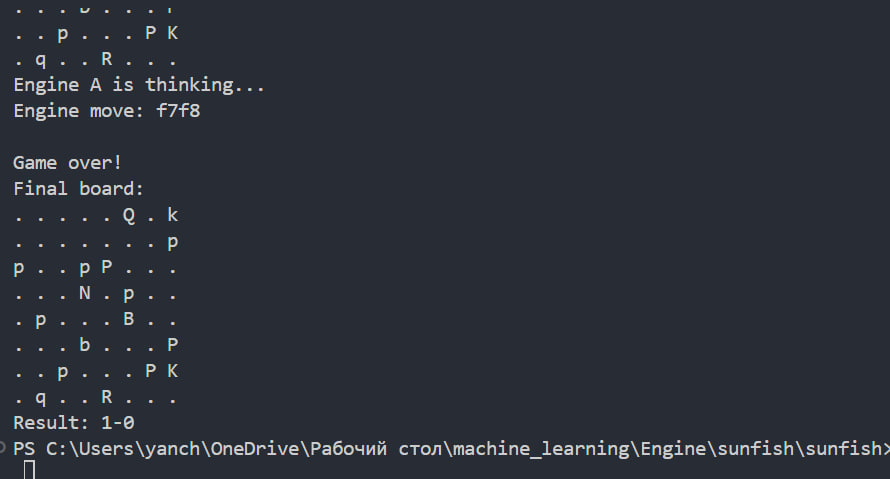
\includegraphics[width=\textwidth]{figures/yanfishwhitemv3000.png}
        \caption{Updated engine (White) wins at 3\,s/move.}
        \label{fig:screenshot1}
        
        \vspace{0.5em}

    \end{subfigure}
    \hfill
    \begin{subfigure}[b]{0.49\textwidth}
        \centering
        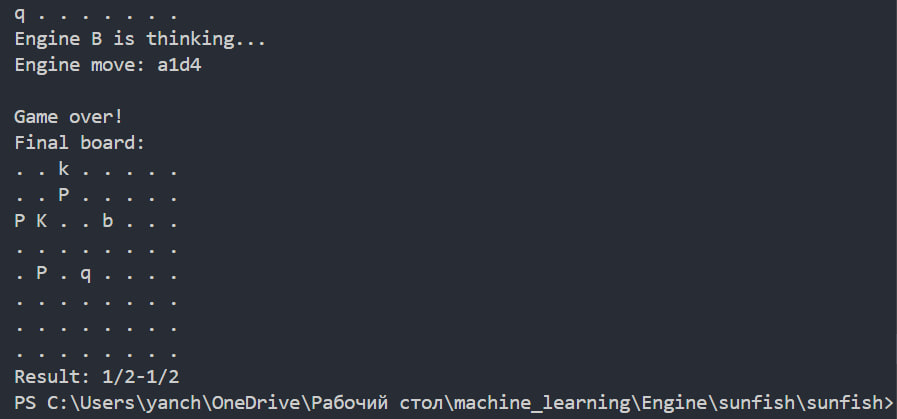
\includegraphics[width=\textwidth]{figures/yanfishblackmv3000.png}
        \caption{Updated engine (Black) draws at 3\,s/move.}
        \label{fig:screenshot2}
        
        \vspace{0.5em}

    \end{subfigure}
    
    \vspace{1em}

    %------------ Row 2 ------------%
    \begin{subfigure}[b]{0.49\textwidth}
        \centering
        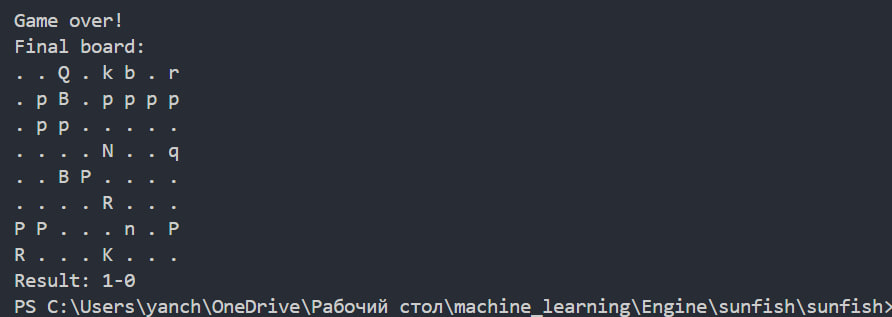
\includegraphics[width=\textwidth]{figures/yanfishwhitedepth1.png}
        \caption{Updated engine (White) wins at depth 1.}
        \label{fig:screenshot3}
        
        \vspace{0.5em}

    \end{subfigure}
    \hfill
    \begin{subfigure}[b]{0.49\textwidth}
        \centering
        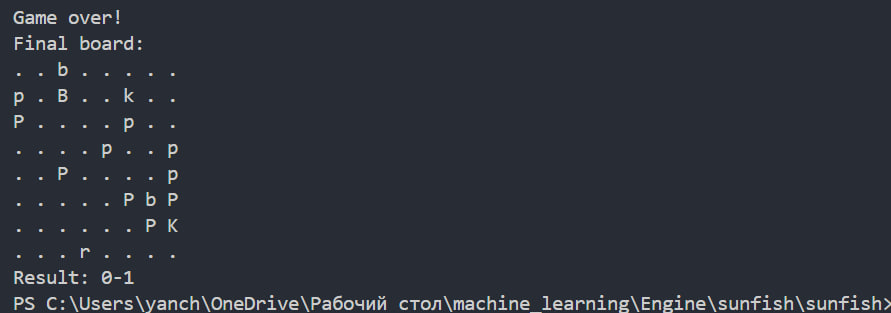
\includegraphics[width=\textwidth]{figures/yanfishblackdepth1.png}
        \caption{Updated engine (Black) wins at depth 1.}
        \label{fig:screenshot4}
        
        \vspace{0.5em}

    \end{subfigure}

    % -- SINGLE CAPTION & LABEL FOR THE ENTIRE SPLIT FIGURE
    
    \label{fig:all_screens_large}
\end{figure}

%========================================================
% SECOND FLOAT (Part 2) -- continues the same figure
%========================================================
\begin{figure}[H]
    \ContinuedFloat  % Tells LaTeX this is still the same figure as above
    \centering
    
    %------------ Row 3 ------------%
    \begin{subfigure}[b]{0.49\textwidth}
        \centering
        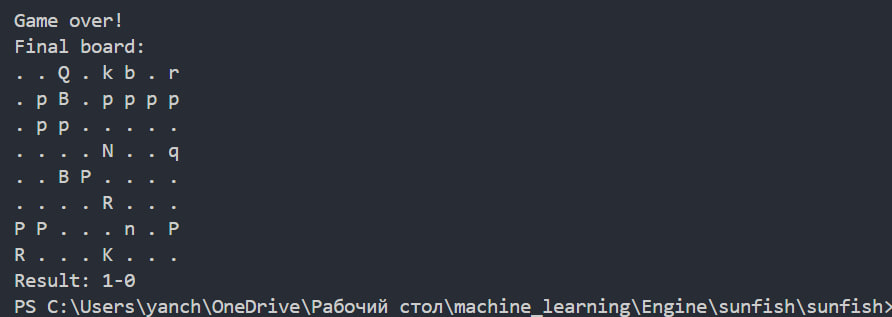
\includegraphics[width=\textwidth]{figures/yanfishwhitedepth1.png}
        \caption{Updated engine (White) at fixed depth 2.}
        \label{fig:screenshot5}
        
        \vspace{0.5em}
        \small

    \end{subfigure}
    \hfill
    \begin{subfigure}[b]{0.49\textwidth}
        \centering
        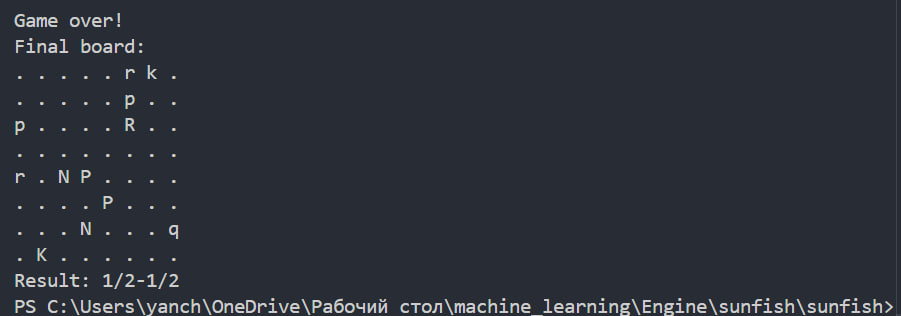
\includegraphics[width=\textwidth]{figures/yanfishblackdepth2.png}
        \caption{Updated engine (Black) draws at fixed depth 2.}
        \label{fig:screenshot6}
        
        \vspace{0.5em}
        \small

    \end{subfigure}

    % -- NO new figure label. We keep the same figure number.
    %    Provide a minimal "continued" note if you like:
    \caption{Six head-to-head match examples between the updated engine and 
             the original Sunfish (two subfigures per row).}
\end{figure}



\subsubsection{Extended Match Results}

A series of \textbf{20 head-to-head games} were played at a move time of \textbf{3 seconds or more} to further examine the updated engine’s performance with longer time controls. Table~\ref{tab:extended_results} summarizes the outcomes:

\begin{table}[ht]
\centering
\begin{tabular}{lcc}
\hline
\textbf{Engine} & \textbf{Wins} & \textbf{Win \%} \\
\hline
Updated Engine   & 13 & 65\% \\
Original Sunfish & 3  & 15\% \\
Draws            & 4  & 20\% \\
\hline
\end{tabular}
\caption{Results from 20 games at 3+ seconds per move.}
\label{tab:extended_results}
\end{table}

With more time to analyze each position, the updated engine leverages its improved evaluation more effectively, winning 65\% of the games against the original Sunfish. Although Sunfish secured 15\% of the wins, the updated approach maintained an advantage in the majority of positions. This outcome suggests that, at slower time controls, the benefit of a stronger evaluation outweighs raw speed, as both engines have enough time to search multiple lines in depth.
\FloatBarrier

\subsection{User Feedback}

User feedback was gathered through a series of informal interviews conducted both in person and via voice calls. These discussions aimed to assess how easily participants could navigate the interface and whether they found the articles enjoyable to read.

From these interviews, three main themes emerged:
\begin{itemize}
    \item \textbf{Navigation Challenges:} A majority of participants reported difficulty navigating the interface, which led to revisions in the final UI design.
    \item \textbf{Complex Content:} Several users felt the articles were difficult to read, prompting further UI refinements to improve clarity and presentation.
    \item \textbf{Positive Responses:} Approximately 30\% of respondents expressed overall satisfaction with the interface, noting no major concerns.
\end{itemize}

These findings influenced multiple aspects of the final version, ensuring that both usability and readability received careful attention.

\subsection{Visualization}
\subsubsection{Maze Visualization Evaluation}
\label{subsec:maze_eval}
The maze visualization was tested with grid sizes ranging from \(20 \times 20\) to \(40 \times 40\). 
In each configuration, the interface successfully displayed the incremental steps of the selected pathfinding algorithm 
(\textit{e.g.}, BFS, DFS, Dijkstra, or A*) and highlighted the final path from the start to the goal cell.

For smaller mazes (\(20 \times 20\)), computations finished almost instantly, allowing the animation to play smoothly. 
As the maze size increased to \(40 \times 40\) or more, a slight delay became noticeable, reflecting the added 
computational load. Nevertheless, users reported the visualization remained helpful in understanding how each algorithm 
expands and prioritizes cells during the search. No instances of crashes or incorrect pathfinding outcomes were observed, 
indicating a robust implementation for typical use cases.

\subsubsection{Minimax Traversal Evaluation}
\label{subsec:minimax_eval}
The minimax traversal was evaluated using a series of chess positions with varying complexity. 
In simpler puzzles featuring only a few possible moves per position, the algorithm performed quickly and accurately, 
often finding the optimal move sequence within a second.

However, in more complex scenarios with a larger branching factor (\textit{e.g.}, mid-game positions containing multiple 
pieces and move options), the exponential growth of the search tree led to noticeable slowdowns at greater depths. 
To address this, \textbf{alpha--beta pruning} was integrated into the minimax routine, 
significantly reducing the total nodes evaluated. 
In tests at a depth of 3 or more, the alpha--beta version evaluated up to 35\% fewer nodes compared to the naive minimax, 
speeding up move discovery. 


%-------------------------------------------------
% Section: Conclusion
%-------------------------------------------------
\section{Discussion}
\subsection{Hypothesis}

The main goal of this project was to create a software tool that addresses the
four questions listed in Section~\ref{sec:hypothesis}. Each point is reviewed
here with an overview of how well it was achieved:

\begin{itemize}[label={}, leftmargin=1em]

\item \textbf{(a)} \textit{Does adding an NNUE-style network to the Sunfish engine
lead to a significant improvement in playing strength, compared to the original
heuristic-based method?}

\item \textbf{(b)} \textit{Can creating a more advanced maze visualization tool
boost clarity, user engagement, and feature completeness beyond what is
currently offered?}

\item \textbf{(c)} \textit{“Could we develop a new tool that interactively visualizes minimax, making the algorithm more understandable?”}

\item \textbf{(d)} \textit{Is it feasible and beneficial to combine NNUE, enhanced
maze visualization, and a minimax visualizer into one platform, offering a
unified set of features to users?}

\end{itemize}

\vspace{0.5em}
\noindent
\textbf{Improvement in Chess Engine Strength (Question (a)).} \\
Tests showed that adding an NNUE-style network to the Sunfish engine did indeed
increase its playing strength. Multiple matches confirmed that the NNUE-enhanced
engine outperforms the original version. This outcome directly answers question (a)
with a clear ``yes,'' as the improved evaluation led to more accurate move choices
and better overall results.

\vspace{0.5em}
\noindent
\textbf{Maze Visualization Enhancements (Question (b)).} \\
The new maze visualization tool includes both random generation and custom
options, which fills the gap mentioned in the literature review. Early versions
received mixed feedback, but subsequent improvements made the interface more
intuitive and comprehensive, thus addressing question (b). The tool now allows
users to explore different maze layouts, track benchmarks, and visually follow the
paths generated by the system.

\vspace{0.5em}
\noindent
\textbf{Minimax Visualizer (Question (c)).} \\
The project also introduced a minimax visualizer that operates independently of
the NNUE engine. In its current form, it utilizes a simple engine to illustrate
how search trees and evaluations are generated in real time. This approach
demonstrates that the visualizer can be adapted to various algorithms or engines,
thus confirming that a real-time minimax view is both feasible and helpful for
understanding decision-making processes.
\vspace{0.5em}
\noindent
\textbf{Combined Platform (Question (d)).} \\
Finally, the updated user interface merges NNUE-based chess analysis, maze
visualization, and the new minimax view into one platform. Although initial UI
designs faced some negative feedback regarding layout and ease of use, the
latest version demonstrates a more unified approach and better user experience.
Therefore, question (d) has largely been met, showing it is both possible and
beneficial to offer all these features together in a single tool.
\subsection{Future Work}

Although this platform offers several useful features, there are many ways to
improve it further:

\begin{itemize}
    \item \textbf{Engine Performance:} Currently, the engine uses a halfkp
    architecture. The original plan was to implement a halfkv2 architecture,
    but it was not successful. It remains unclear whether the issue lies in the
    code or the weights themselves. Investigating this problem and moving to
    halfkv2 in the future could significantly boost engine strength.

    \item \textbf{Maze Input and Analysis:} In the maze-solving component,
    allowing users to upload images that an AI agent converts into mazes
    could be very helpful, especially for individuals working on robotics or
    pathfinding research. This feature would allow greater flexibility and
    more real-world applications.

    \item \textbf{Minimax Visualizer Integration:} At present, the minimax
    visualizer uses a simple engine to demonstrate how search trees and
    evaluations are generated. Integrating this visualizer with a more advanced
    engine (such as the NNUE-enhanced version) would give users deeper insight
    into the decision-making process during actual gameplay.

    \item \textbf{Platform Expansion:} While the current platform supports
    essential features, there is potential to extend its capabilities even
    further. Future updates might include more comprehensive visualizations
    for both maze generation and the chess engine. This could involve showing
    additional metrics, more interactive controls, or support for other AI
    techniques, allowing the platform to grow into a fully featured research
    and learning tool.
\end{itemize}

By pursuing these directions, the platform can continue to evolve, serving as
both a more powerful chess engine and a more flexible maze and decision-making
visualization environment.

\subsection{Conclusion}
\label{sec:conclusion}
This project combined three important components: a stronger chess engine, an improved maze visualization tool, and a minimax visualizer. The chess engine was enhanced by incorporating a neural network (NNUE-style), leading to better overall play. The maze tool allows users to generate random or custom layouts, simplifying the study of various paths and designs. Meanwhile, the minimax visualizer displays the engine’s decision-making process step by step, giving a clear look into how the search works. Having these features all in one platform offers a more engaging learning environment for both chess and pathfinding. Future goals include further strengthening the chess engine, introducing additional maze customization options, and integrating the minimax visualizer with the advanced engine to deliver an even more comprehensive experience.
% references section


\bibliographystyle{IEEEtran}
\bibliography{references} 
%-------------------------------------------------
% Appendix (Optional in article)
%-------------------------------------------------
\appendix
\section{Appendix}
\label{sec:appendix}

This appendix presents additional screenshots from the application’s user interface. 
Each figure has a short caption, and the paragraphs below highlight key features 
or functionalities shown in each image.

%-----------------------------------------
\begin{figure}[htbp]
  \centering
  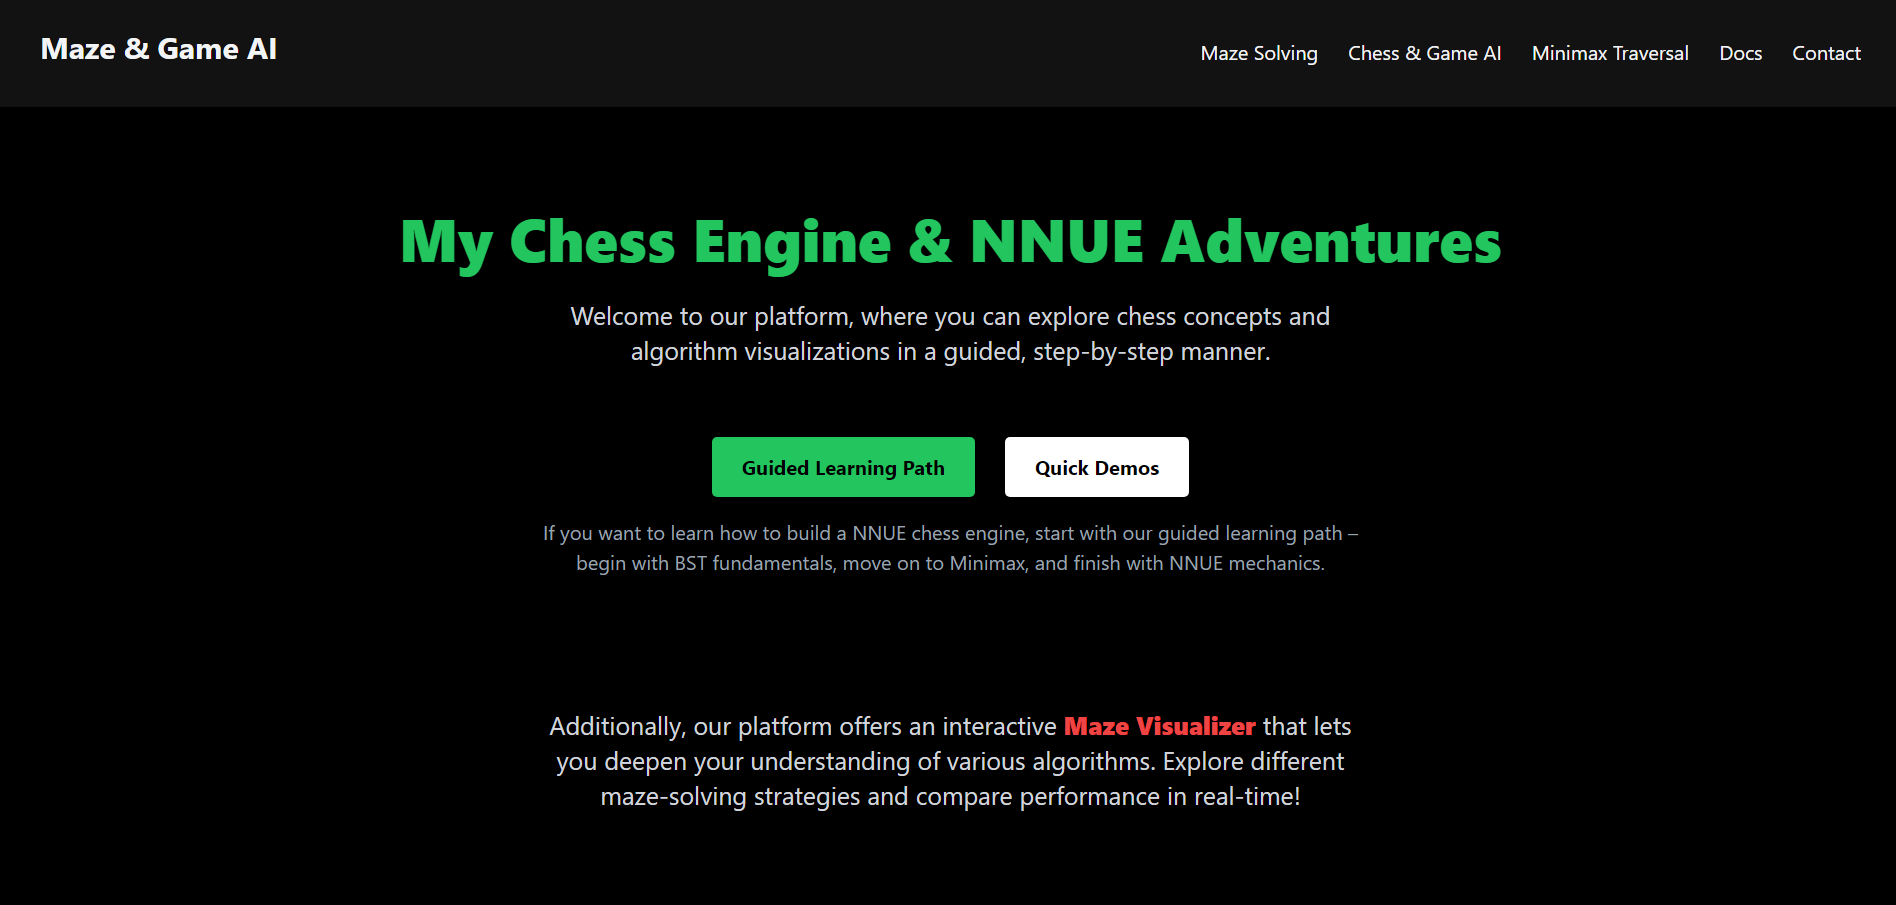
\includegraphics[width=0.9\textwidth]{figures/Main.png}
  \caption{Main interface showing the navigation bar and welcome message (part of the \texttt{mainpage} component).}
  \label{fig:ui_main_screen}
\end{figure}

\noindent
Figure~\ref{fig:ui_main_screen} shows the \emph{main homepage layout}, 
including a welcome message and a navigation bar for exploring different features.

\FloatBarrier
%-----------------------------------------
\begin{figure}[htbp]
  \centering
  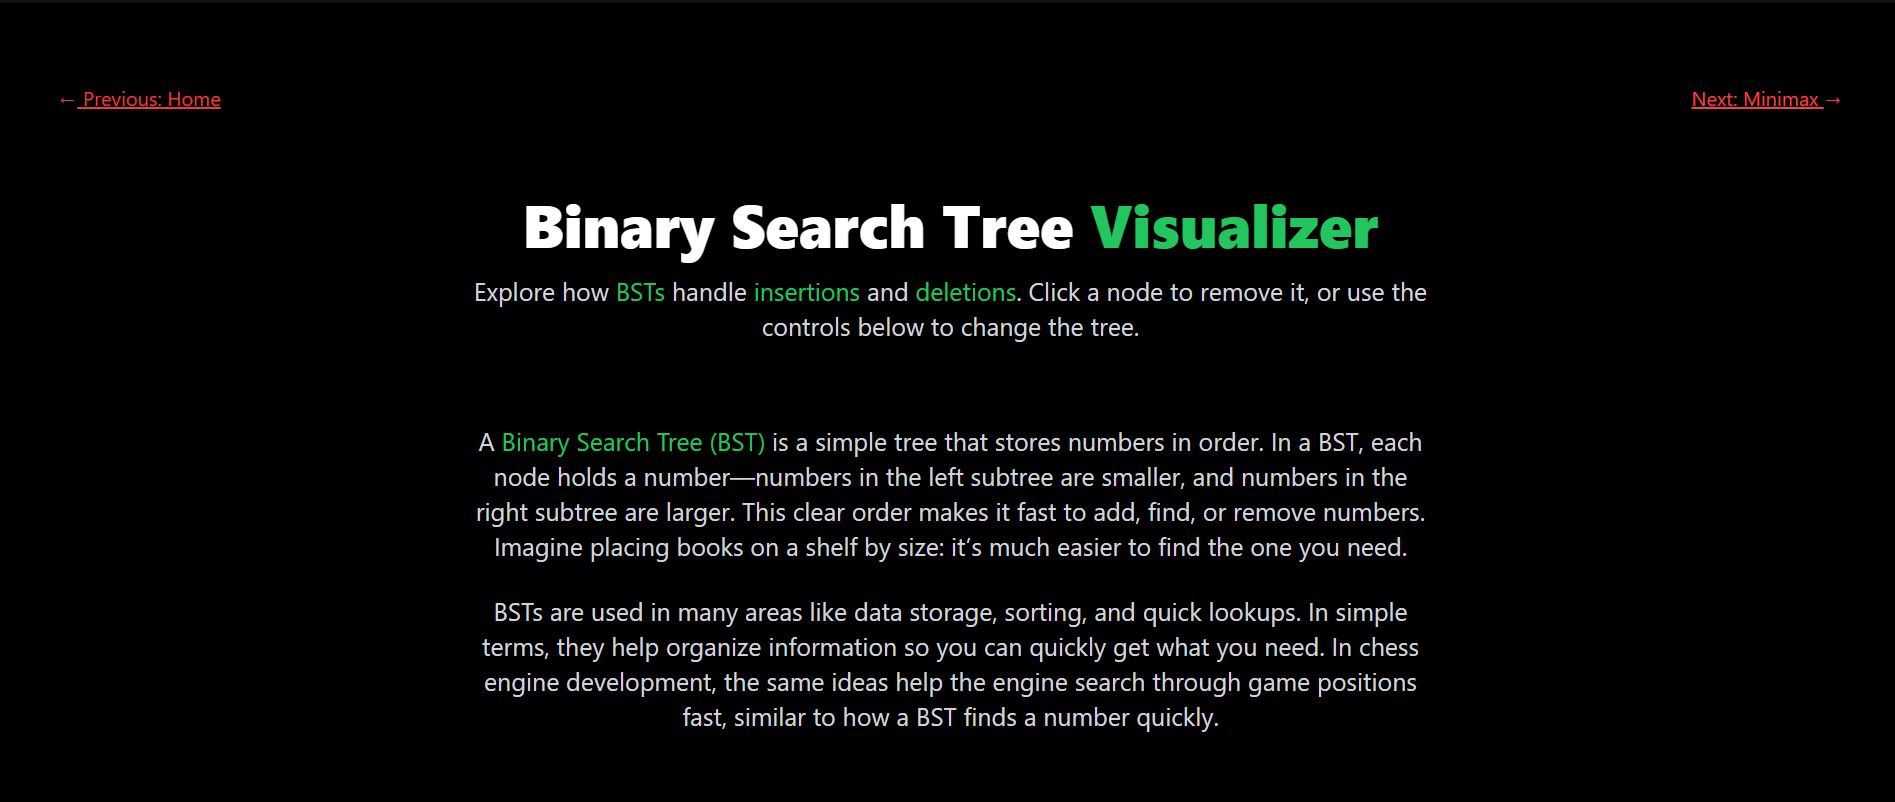
\includegraphics[width=0.9\textwidth]{figures/Bst.png}
  \caption{Guided path for users interested in building an NNUE (Neural Network Updatable Engine).}
  \label{fig:bst}
\end{figure}

\noindent
Figure~\ref{fig:bst} illustrates part of a guided path where beginners 
can follow step-by-step instructions to construct an NNUE-based chess engine.

\FloatBarrier
%-----------------------------------------
\begin{figure}[htbp]
  \centering
  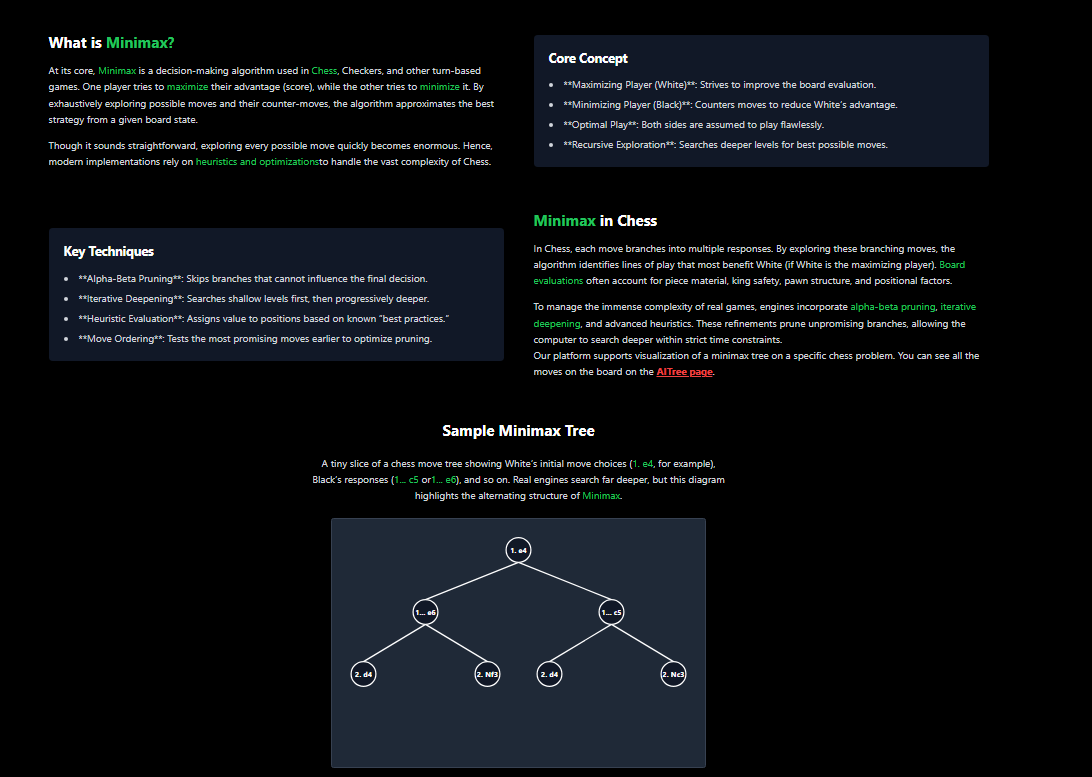
\includegraphics[width=0.9\textwidth]{figures/Minimaxguided.png}
  \caption{Minimax page from a guided path.}
  \label{fig:minimaxguided}
\end{figure}

\begin{figure}[htbp]
  \centering
  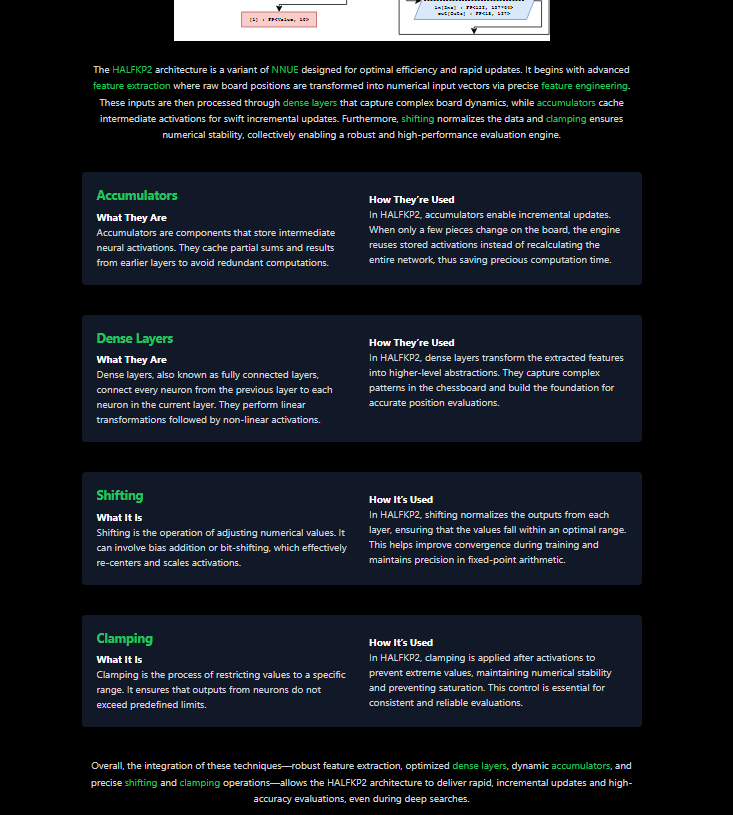
\includegraphics[width=0.9\textwidth]{figures/Nnnueguided.png}
  \caption{NNUE page from a guided path (fully zoomed out).}
  \label{fig:nnueguided}
\end{figure}

\noindent
Figures~\ref{fig:minimaxguided} and \ref{fig:nnueguided} capture other guided 
pages. The first focuses on step-by-step minimax explanations, while the second 
covers building an NNUE engine in greater depth.

\FloatBarrier
%-----------------------------------------
\begin{figure}[htbp]
  \centering
  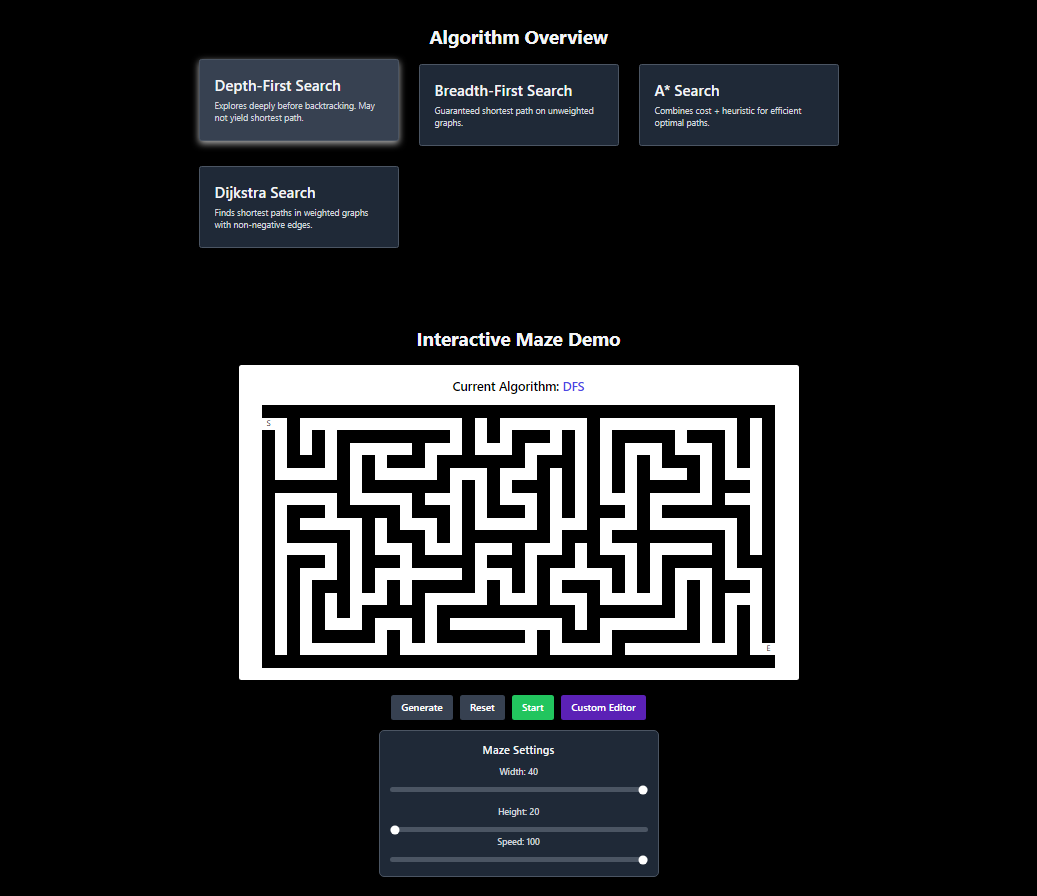
\includegraphics[width=0.9\textwidth]{figures/mazesolvingmain.png}
  \caption{Top portion of the \texttt{mazesolving} component, showing algorithm selection, maze area, and a control panel with settings.}
  \label{fig:mazesolvingmain}
\end{figure}

\begin{figure}[htbp]
  \centering
  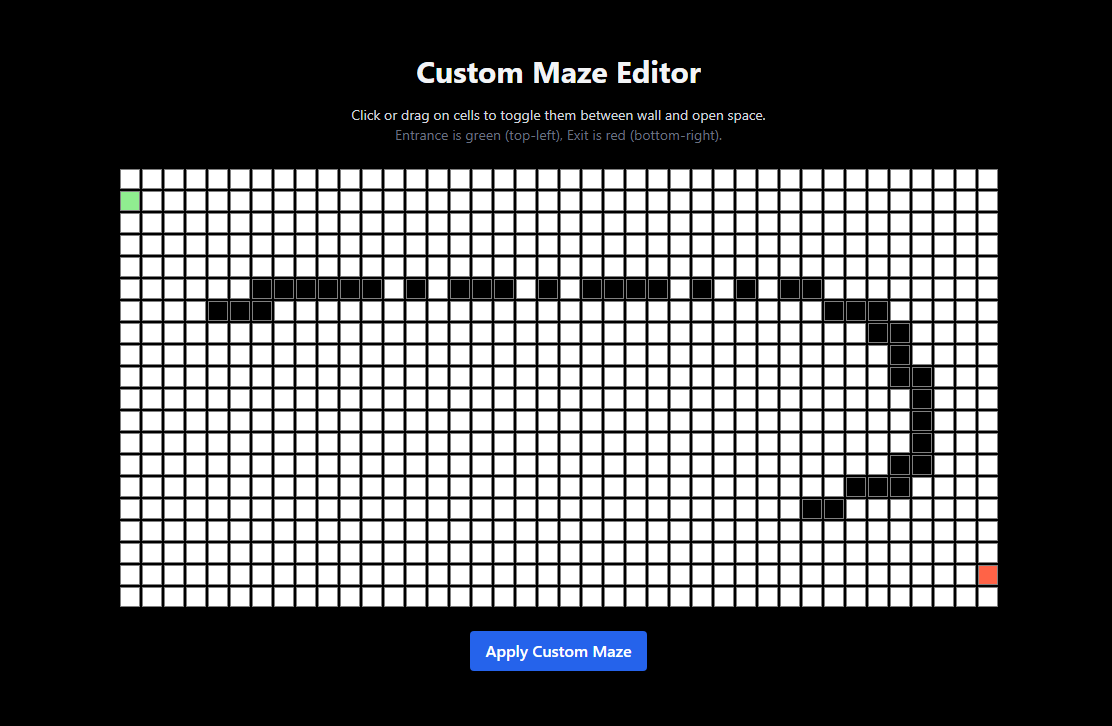
\includegraphics[width=0.9\textwidth]{figures/Custommaze.png}
  \caption{Section of the \texttt{mazesolving} component for building a custom maze.}
  \label{fig:custommaze}
\end{figure}

\noindent
Figure~\ref{fig:mazesolvingmain} displays the upper section of the \texttt{mazesolving} 
component, including controls or parameters for selecting various pathfinding algorithms.  
Figure~\ref{fig:custommaze} shows how users can manually construct maze walls and pathways 
to explore unique pathfinding scenarios.

\FloatBarrier
%-----------------------------------------
\begin{figure}[htbp]
  \centering
  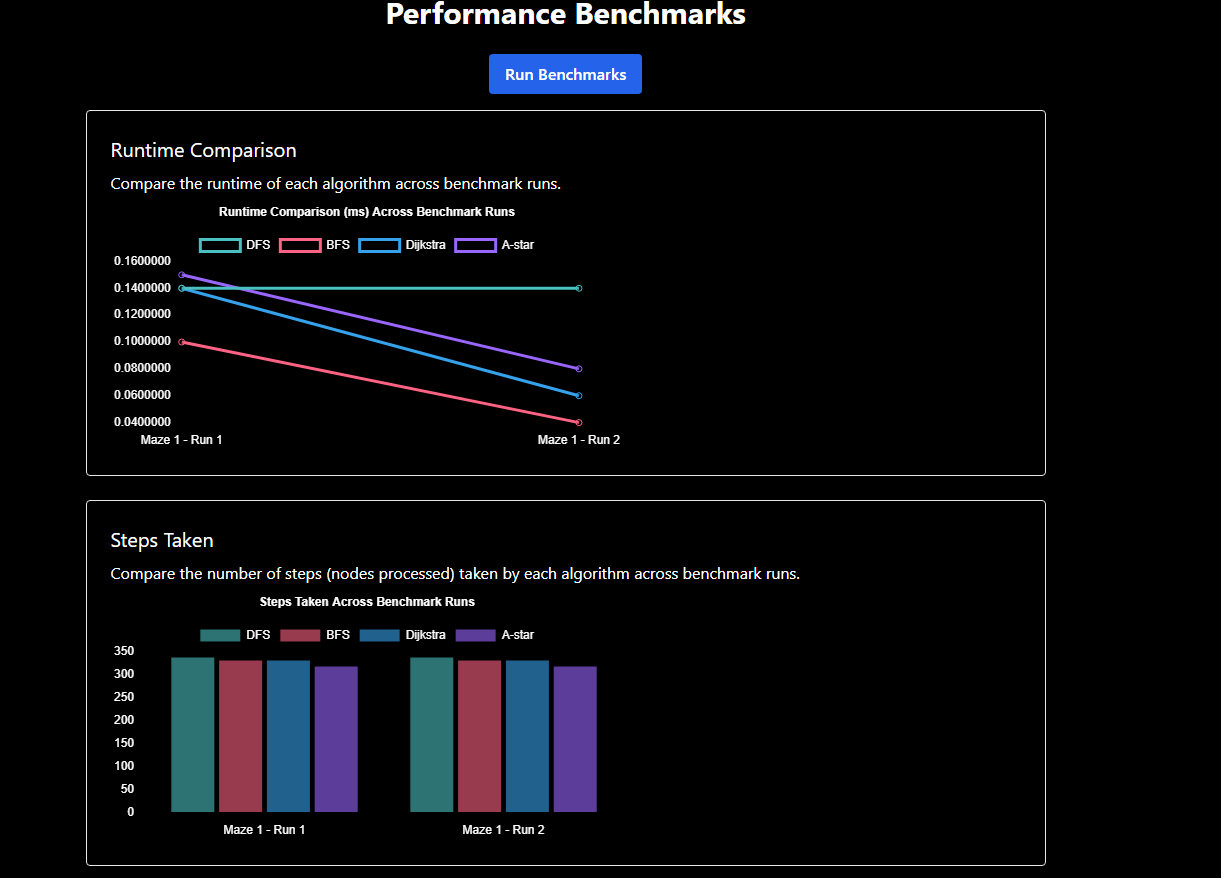
\includegraphics[width=0.9\textwidth]{figures/Benchmarks.png}
  \caption{Benchmarks section within the \texttt{mazesolving} component.}
  \label{fig:benchmarks}
\end{figure}

\noindent
Figure~\ref{fig:benchmarks} shows benchmark results to help users compare the 
performance of different pathfinding methods under various conditions.

\FloatBarrier
%-----------------------------------------
\begin{figure}[htbp]
  \centering
  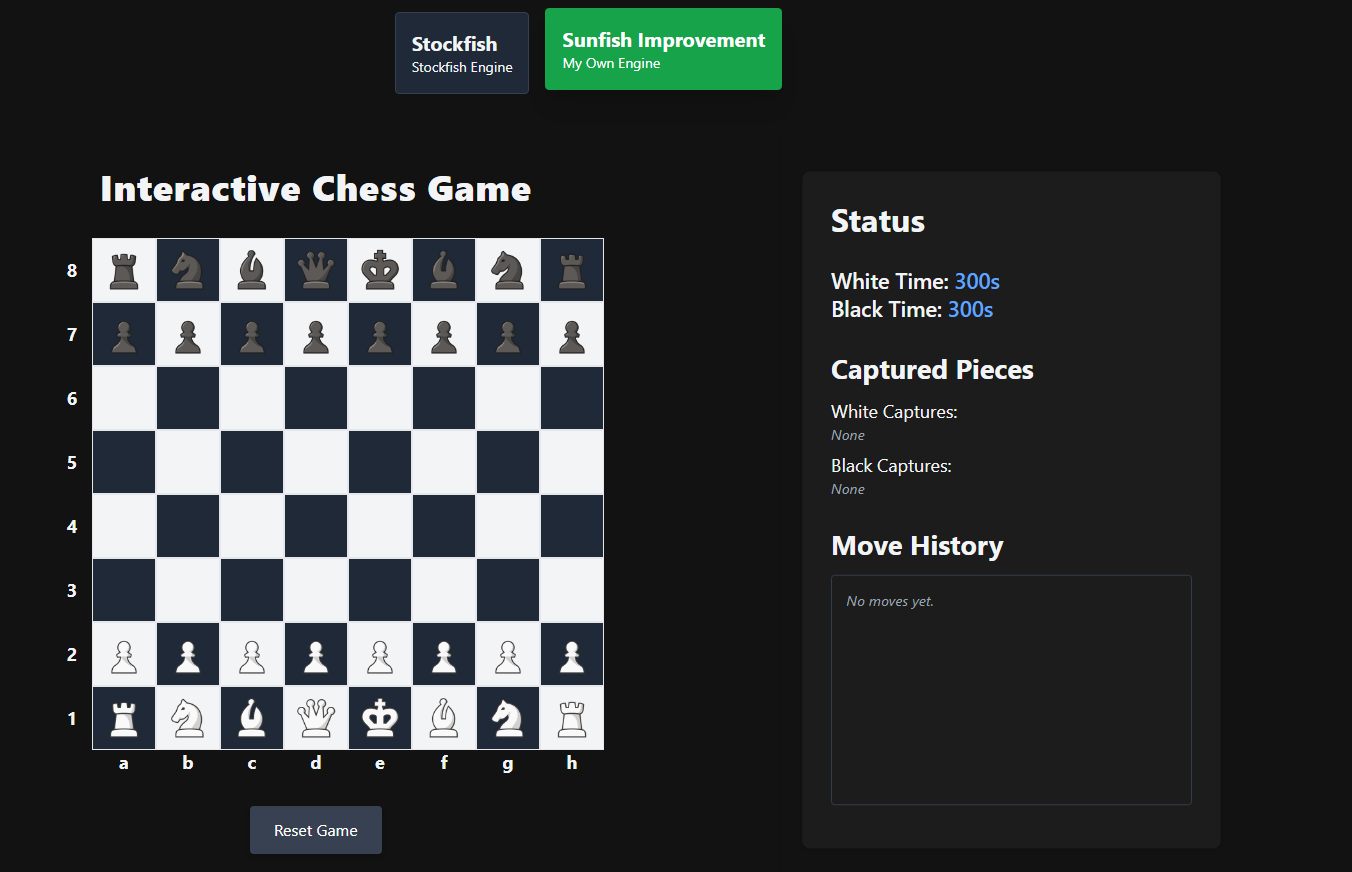
\includegraphics[width=0.9\textwidth]{figures/Chessplay.png}
  \caption{\texttt{chessgame} component where users can play against the updated engine or Stockfish.}
  \label{fig:chessplay}
\end{figure}

\noindent
Figure~\ref{fig:chessplay} depicts the \texttt{chessgame} interface, 
allowing users to switch between Stockfish or the custom NNUE-based engine, 
review a move history, manage time controls, and more.

\FloatBarrier
%-----------------------------------------
\begin{figure}[htbp]
  \centering
  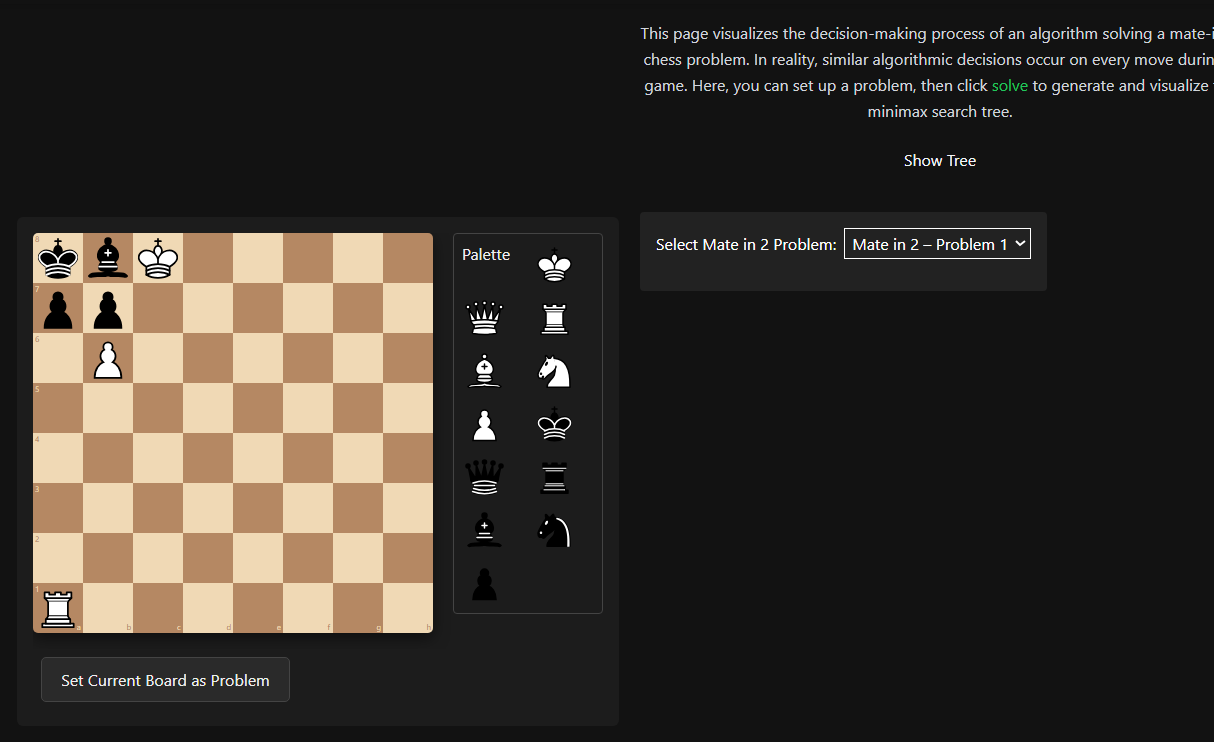
\includegraphics[width=0.9\textwidth]{figures/Minimaxpageinitial.png}
  \caption{Initial state of the \texttt{minimaxsolver} component.}
  \label{fig:minimaxinitial}
\end{figure}

\noindent
Figure~\ref{fig:minimaxinitial} shows how the \texttt{minimaxsolver} begins 
with a default chess position ready to be analyzed or changed by the user.

\FloatBarrier
%-----------------------------------------
\begin{figure}[htbp]
  \centering
  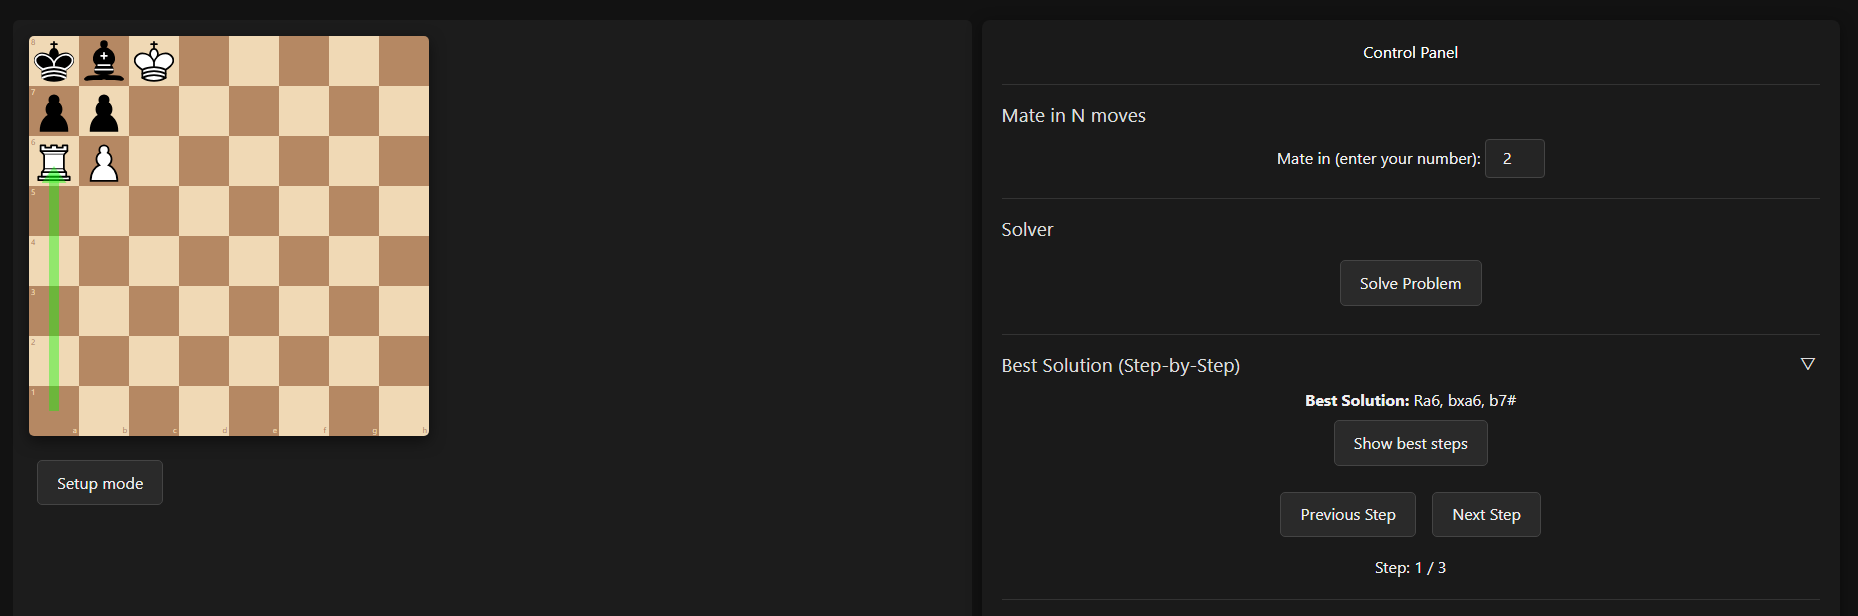
\includegraphics[width=0.9\textwidth]{figures/Minimaxafterplay.png}
  \caption{\texttt{minimaxsolver} component after a problem is set up and partially solved.}
  \label{fig:Minimaxafterplay}
\end{figure}

\noindent
In Figure~\ref{fig:Minimaxafterplay}, the minimax algorithm is actively searching 
once the user defines a particular chess position or puzzle to solve.

\FloatBarrier
%-----------------------------------------
\begin{figure}[htbp]
  \centering
  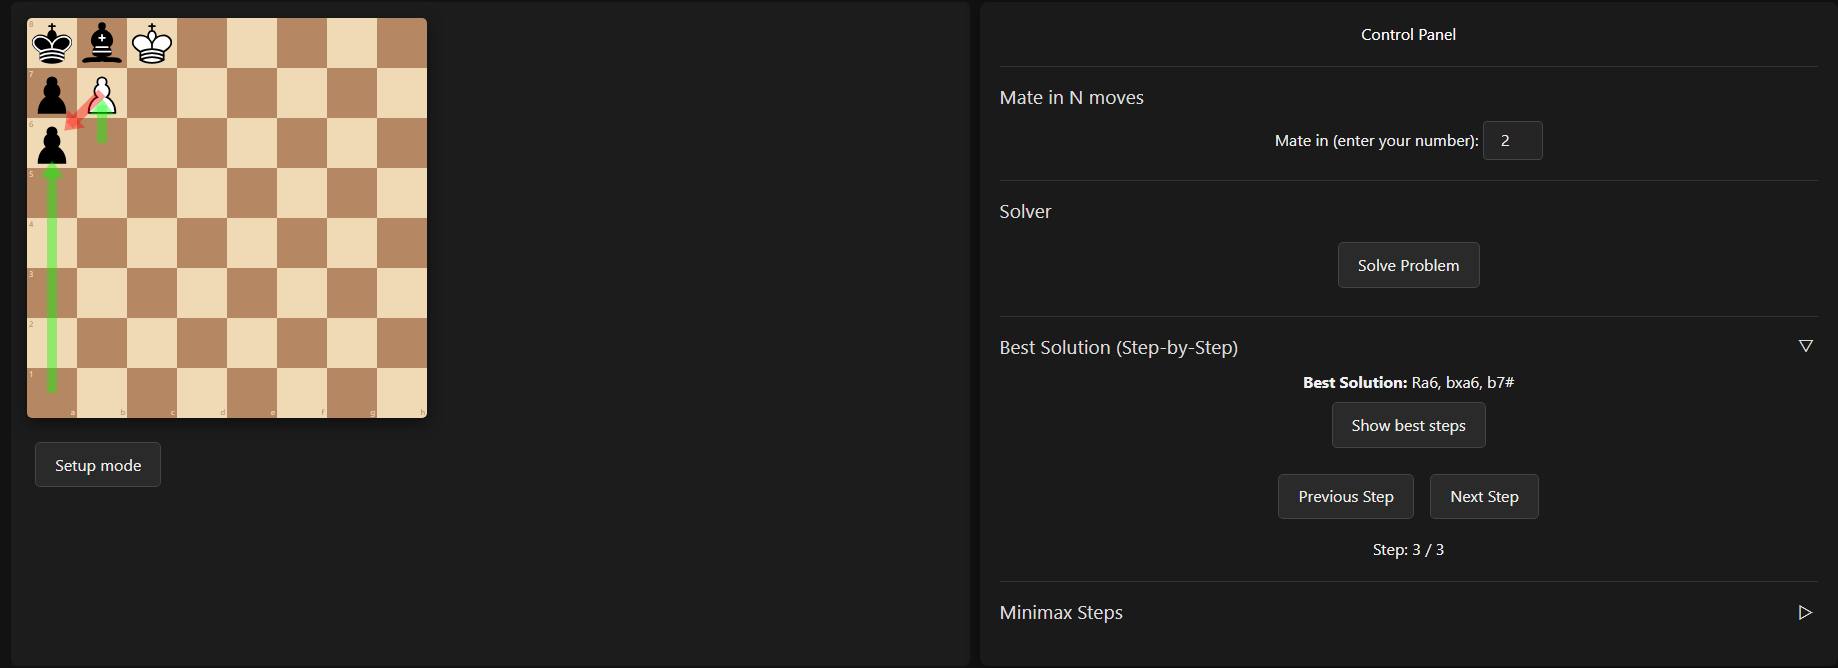
\includegraphics[width=0.9\textwidth]{figures/Minimaxfinish.png}
  \caption{\texttt{minimaxsolver} component after the problem is fully traversed.}
  \label{fig:minimaxfinished}
\end{figure}

\noindent
Figure~\ref{fig:minimaxfinished} depicts the state once minimax completes 
its search and outputs a final evaluation or sequence of moves.

\FloatBarrier
%-----------------------------------------
\begin{figure}[htbp]
  \centering
  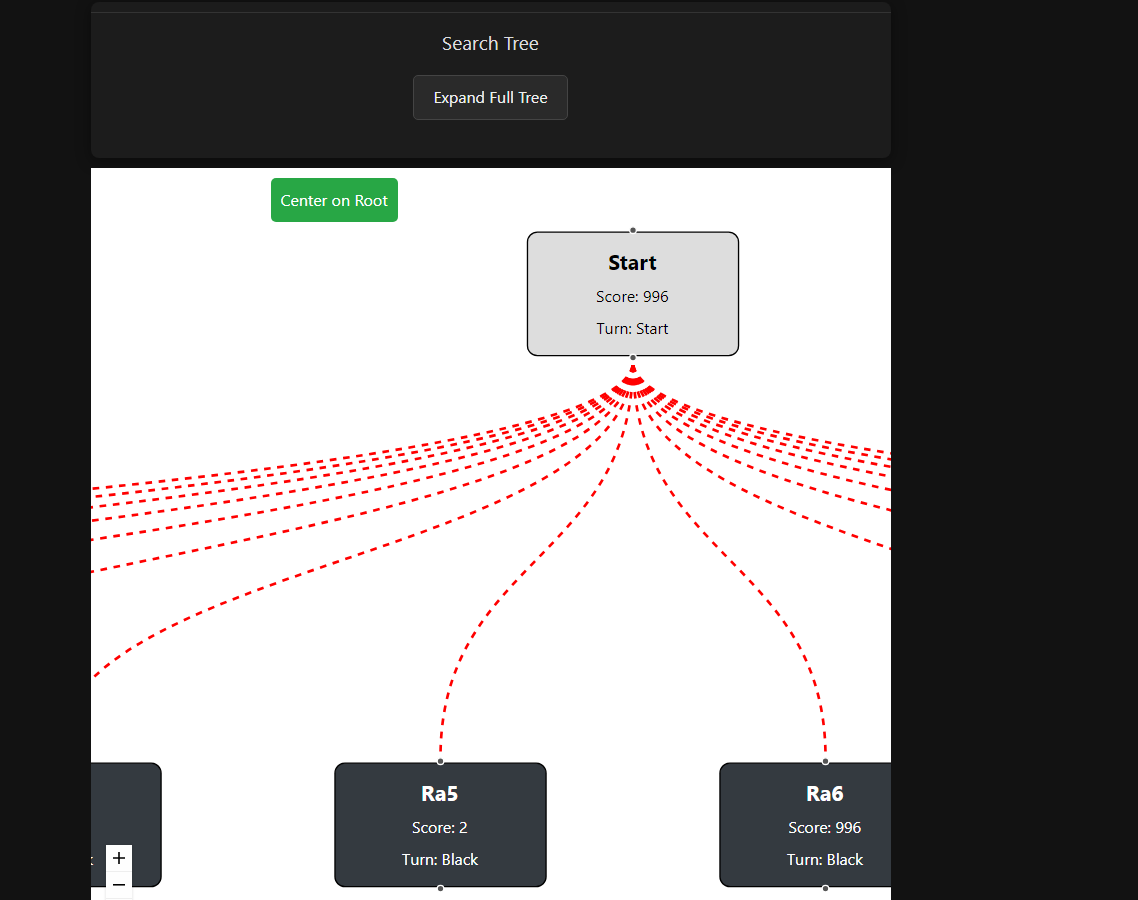
\includegraphics[width=0.9\textwidth]{figures/MInimaxtree.png}
  \caption{Example of the search tree generated by \texttt{minimaxsolver} for a given chess puzzle.}
  \label{fig:minimaxtree}
\end{figure}

\noindent
Figure~\ref{fig:minimaxtree} displays the expanded search tree where each node 
corresponds to a possible move or outcome during minimax exploration.

\FloatBarrier
%-----------------------------------------
\begin{figure}[htbp]
  \centering
  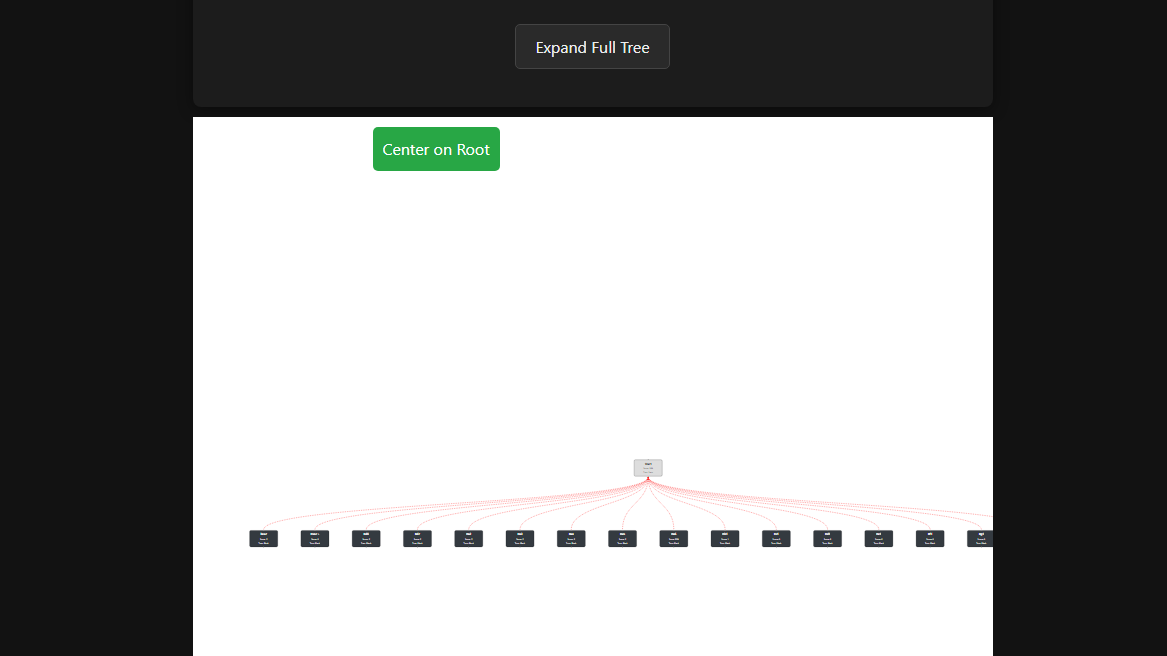
\includegraphics[width=0.9\textwidth]{figures/treefinal.png}
  \caption{An expanded, zoomed-out view of the \texttt{minimaxsolver} tree.}
  \label{fig:minimaxtreefinal}
\end{figure}

\noindent
Finally, Figure~\ref{fig:minimaxtreefinal} shows a zoomed-out perspective of the 
search tree, highlighting how nodes can be expanded or collapsed for closer inspection.

\FloatBarrier
%-----------------------------------------

\noindent
These screenshots, combined with the main text discussion, should help readers 
visualize the user interface and understand how each component operates, 
whether it is the \texttt{mazesolving} section, the \texttt{chessgame} environment, 
or the \texttt{minimaxsolver} module.


\end{document}




